   %---------------- COMMENT FOR IMPORTING ----------------------
%\RequirePackage{lineno}				
%\documentclass[12pt]{report}		
%\pagestyle{headings}
%\input{ST-input2}							

%\setcounter{chapter}{0}
%\begin{document}								
%\setpagewiselinenumbers
%\linenumbers
%\tableofcontents
\graphicspath{{Chapter3/figures/}} 
%-------------------------------------------------------------

\chapter{Identifying corruption within acoustic sensing signals}
\label{chap:das}

\section{Introduction}
\label{sec:das_intro}

In Chapter \ref{chap:spectral} we introduced the CluStream \citep{Aggarwal2003} algorithm and demonstrated how it could be used to create an online spectral clustering algorithm. In this chapter we apply CluStream to identify corruption within acoustic sensing signals.  Distributed acoustic sensing (DAS) is a modern technique used to monitor oil flow at various depths throughout an oil  well. DAS uses a fibre-optic cable to record vibrations at very high resolutions, up to 10000 observations a second.  DAS is fairly cheap to implement and offers high frequency data, but unfortunately corruption can occur in the signal.  Our challenge is to identify the locations in the signal where corruption occurs. Existing methods for detecting and removing interference in DAS signals involve using offline, univariate changepoint detection. However DAS signals are multivariate and require online processing. In this chapter we show that CluStream  provides an alternative approach to  changepoints analysis to identify corruption within DAS signals.

\section{Motivation}
\label{sec:das_motivation}

\subsection{What is Distributed Acoustic Sensing?}

Distributed Acoustic Sensing (DAS) is a technique which uses fibre-optic cables to measure vibrations travelling through the ground. DAS systems have recently become popular in the oil and gas industry  and are used to monitor oil flow \citep{Silkina2014, VanderHorst2014} and to detect leaks in abandoned gas wells \citep{Boone2014}. When vibrations pass through the fibre-optic cable, they induce a change in the intensity of the reflection of the pulses of light being passed through the cable. This provides very high frequency data, potentially as high as 10kHz. It is also possible to collect this data at many different depths in the well simultaneously. Therefore DAS data has both high frequency and high dimensionality.

\begin{figure}[h]
   \centering
   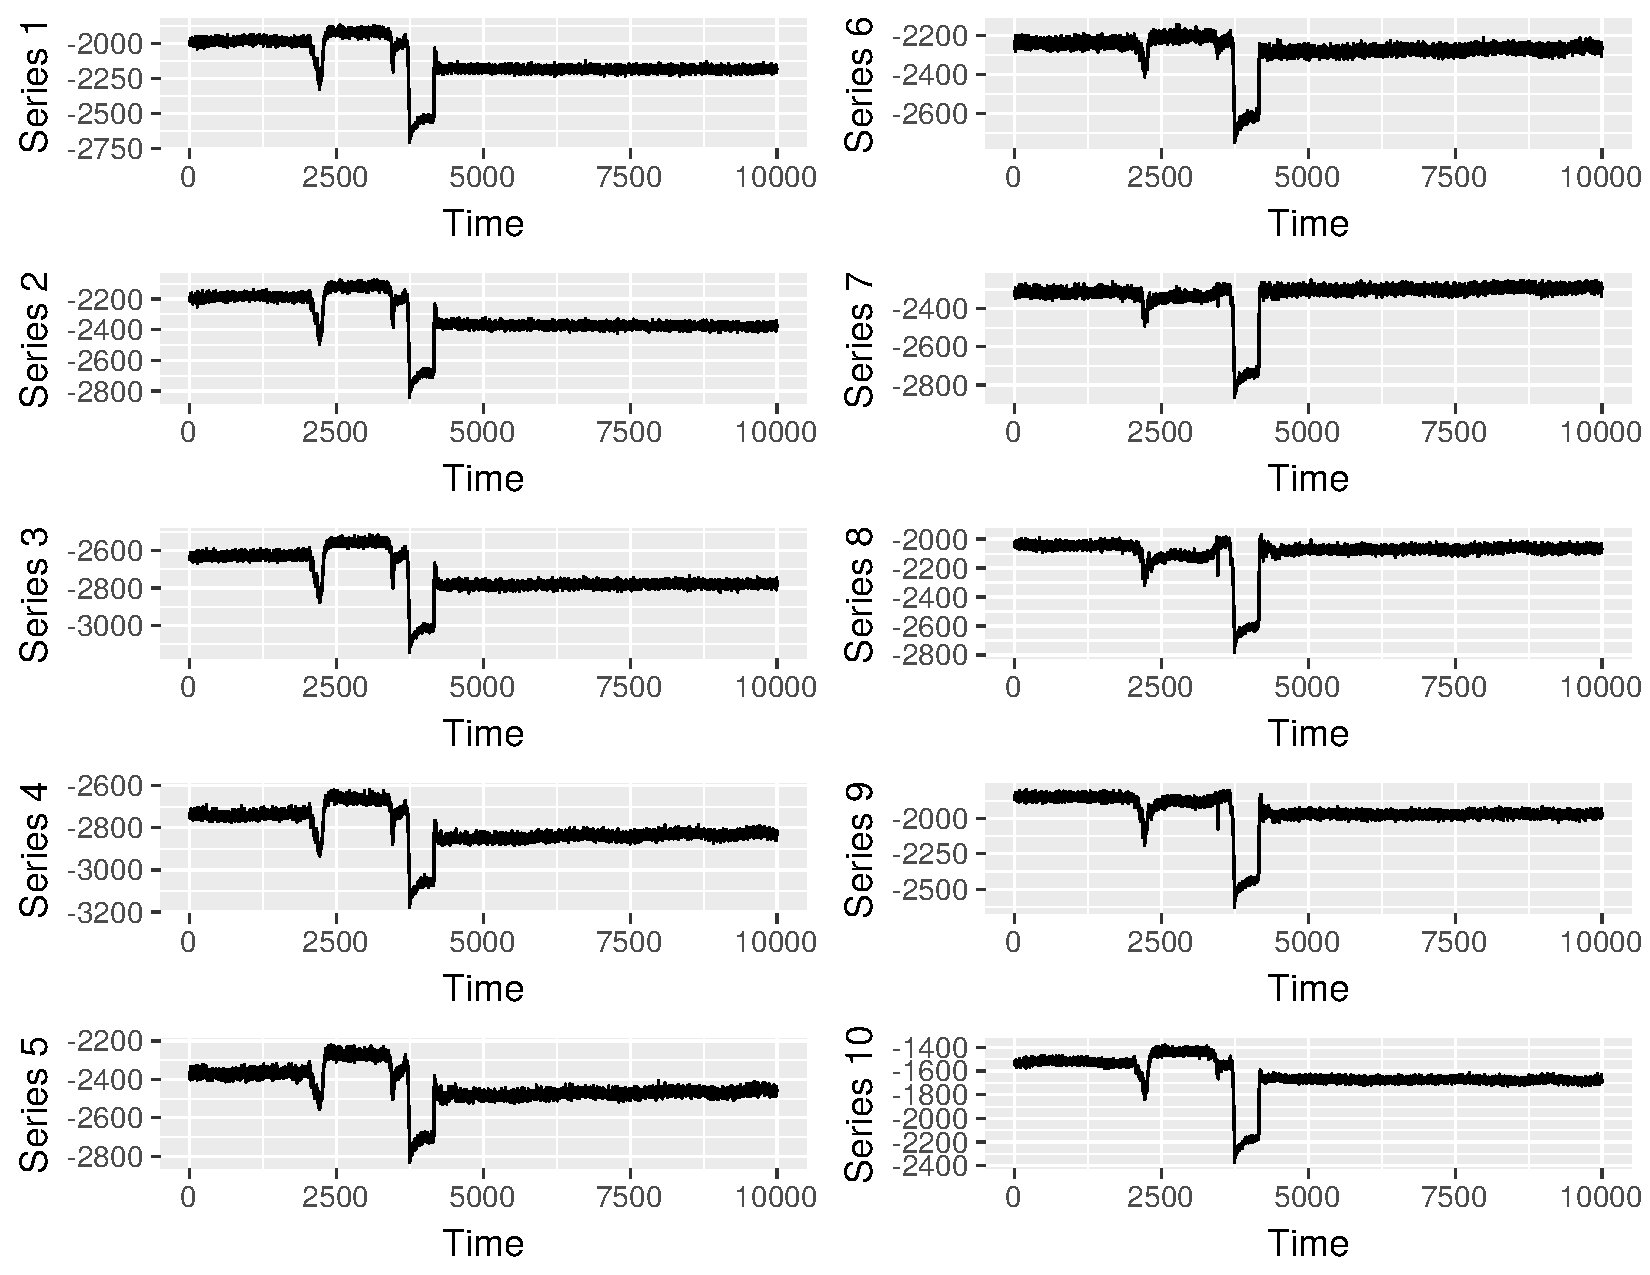
\includegraphics[width = 14cm]{multiplot_wider_new} 
   \caption{An example of acoustic sensing data observed at various depths in an oil well. }
   \label{fig:oil_example}
 \end{figure}

An example of DAS signal data is given in Figure \ref{fig:oil_example}. In the figure, each plot is a series obtained at a different depth within the oil well. We can  see that there are some disturbances in the signal. Engineers refer to these disturbances as corrupted data and the challenge of this application is to locate where the data is corrupted. We are told that if corruption is observed at one depth then the effect is also likely to be observed at multiple other depths simultaneously. This is visible in Figure \ref{fig:oil_example}, particularly at time point $t =  3750$, where there is a big drop in the signal which occurs in all ten series.

\subsection{Relevant literature}

Detecting corruption within a time series is usually framed as a changepoint detection problem. A changepoint is defined as a time-point at which a change occurs in one or more of the statistical properties of a time series. The first published article concerning changepoints was in \cite{Page1954} which considered testing for a potential single changepoint and was motivated by a quality control setting in manufacturing. Over the decades, changepoint analysis has developed rapidly with multiple changepoints, different types of data and other assumptions being considered. Many methods for detecting changepoints exist ranging from approximate (heuristic) fast methods, to exact methods which take longer to run. A review of recent changepoint methods can be found in \cite{Chen2012,Eckley2011b}.

Much of the work in changepoint detection has focused on the scenario where the observations are univariate, although some extensions have been developed for the multivariate setting. The available changepoint algorithms which are multivariate cannot currently deal with the online scenario due to computational restraints. However due to the high frequency and dimensionality of DAS data, an online method is required. 

%The simplest version is detecting whether there is a single changepoint or not. This is framed as a hypothesis test using a general likelihood ratio. binary segmentation \cite{Maidstone2016}.such as the PELT method of \cite{Killick2012} %WBS method  \citep{Fryzlewicz2014}%Some dynamic programming Most methods are offline. There is a need for online.Online changepoint methods \cite{Hawkins2010}

\subsection{Using  CluStream to identify boundary locations}

We consider the problem of identifying corruption within a DAS data stream as a two-stage clustering problem. The first stage is purely online, and consists of updating micro-clusters as a way of storing information about the data stream without storing all of the data points.  The second stage is applied on a small, recent section of the data stream, and allows the user to request a segmentation of that section of the stream to look for where the signal is corrupted. 
\subsection{Stage one: Micro-clustering}
\label{sec:das_stage_1}

Stage one is essentially the micro-clustering step of CluStream introduced in Section \ref{sec:microSpec}.  CluStream is a method of clustering data streams, based on the concept of micro-clusters. Micro-clusters are data structures which summarise a set of instances from the stream, and are composed of a set of statistics which are easily updated and allow fast analysis.  The number of micro-clusters used is a user chosen parameter. Using a large number of micro-clusters will represent the data stream better than a smaller number, at the cost of increased computation. We found using 250 micro-clusters to be sufficient for this application. 
%The statistics we track are defined in equation \eqref{eq:microcluster_def}, $\boldsymbol{CF1^x_j}$ is the sum of all observed data in micro-cluster $j$, $\boldsymbol{CF2^x_j}$ is the sum of the squares of the data and $n_j$ is the number of elements assigned to that micro-cluster. $CF1^t_j$ and $CF2^t_j$ refer to the sum of the time stamps, and the sum of squared time stamps respectively.
\subsection{Stage two: Identifying corruption}
\label{sec:das_stage_2}

Stage two is an offline procedure which is performed in batch on a recent section of the signal. This step uses the micro-cluster summaries to identify a set $B$ of \textit{boundary locations}, points in the signal where there is a change in the signal. First the k-means algorithm is applied on the micro-cluster centres. The clusters generated by the k-means step are referred to as macro-clusters. Then we consider the  $N$ most recently observed data points in the signal, $\{ x_1, ..., x_N \}$. Each of these $N$ points is assigned to a k-means macro-cluster using the nearest neighbour algorithm. We can now plot the signal coloured by the macro-cluster assignments. An example of this is given in Figure \ref{fig:das_kmeans_col}.  

\begin{figure}[h]
  \centering
  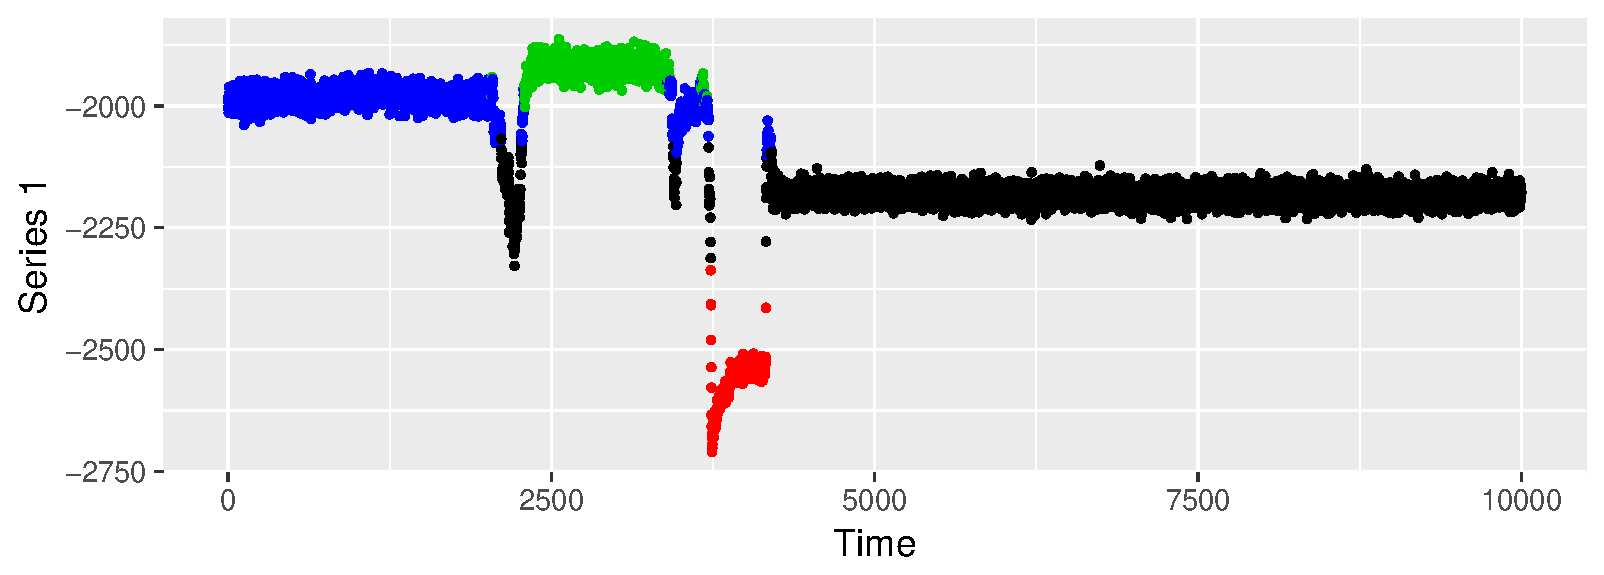
\includegraphics[width = 13cm]{k_4_rep_1_series_1_new.pdf}
  \caption{Series one of the DAS data coloured by macro-cluster assignments.}
  \label{fig:das_kmeans_col}
\end{figure}

Informally, it appears that we can visualise where a change in structure occurs as indicated by the change in cluster assignment. In Figure \ref{fig:das_kmeans_col} this is shown as a change in the colour of the signal. However, we would like to output a set of locations in time where change occurs. Note that during the clustering steps, we do not use the timestamps as input to the clustering. This means that we do not specifically tell the clustering to consider points closer in time as more similar. As a result, there is not necessarily a clear change in the cluster assignments.
The method that we use to convert the clustering of assignments into a set of boundary locations is as follows. Consider a data point in $\{ x_1, ..., x_N \}$, lets call it $\tau$. In order to decide whether it is likely to be a boundary point we consider the k-means assignments of the data points directly before $\tau$ and directly after $\tau$. If the assignments of those points are different, $\tau$ is likely to be a boundary location, if the assignments either side of $\tau$ are similar then $\tau$ is not likely to be a boundary location. The number of data points we look either side of $\tau$ is given by the search parameter $\gamma$. A simple example is shown in Figure \ref{fig:change_in_mean}.

\begin{figure}[H]
  \centering
  \begin{subfigure}{0.48\textwidth}
    \centering
    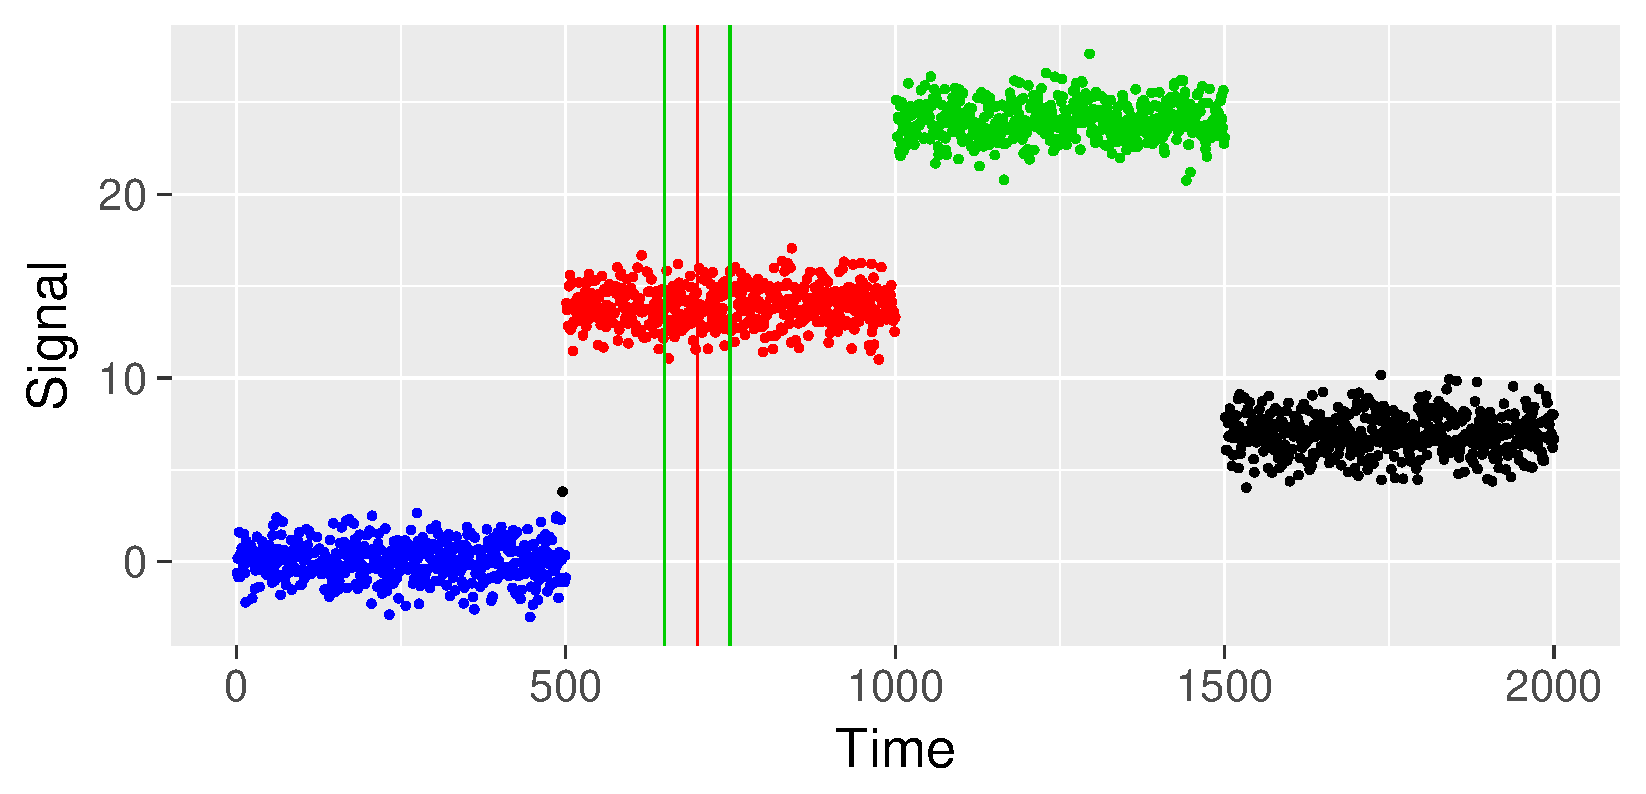
\includegraphics[width = \textwidth]{cim_6_new}
    \caption{$\tau = 700 $, $\gamma = 50.$}
  \label{fig:cim_6}
  \end{subfigure}
  \begin{subfigure}{0.48\textwidth}
    \centering
    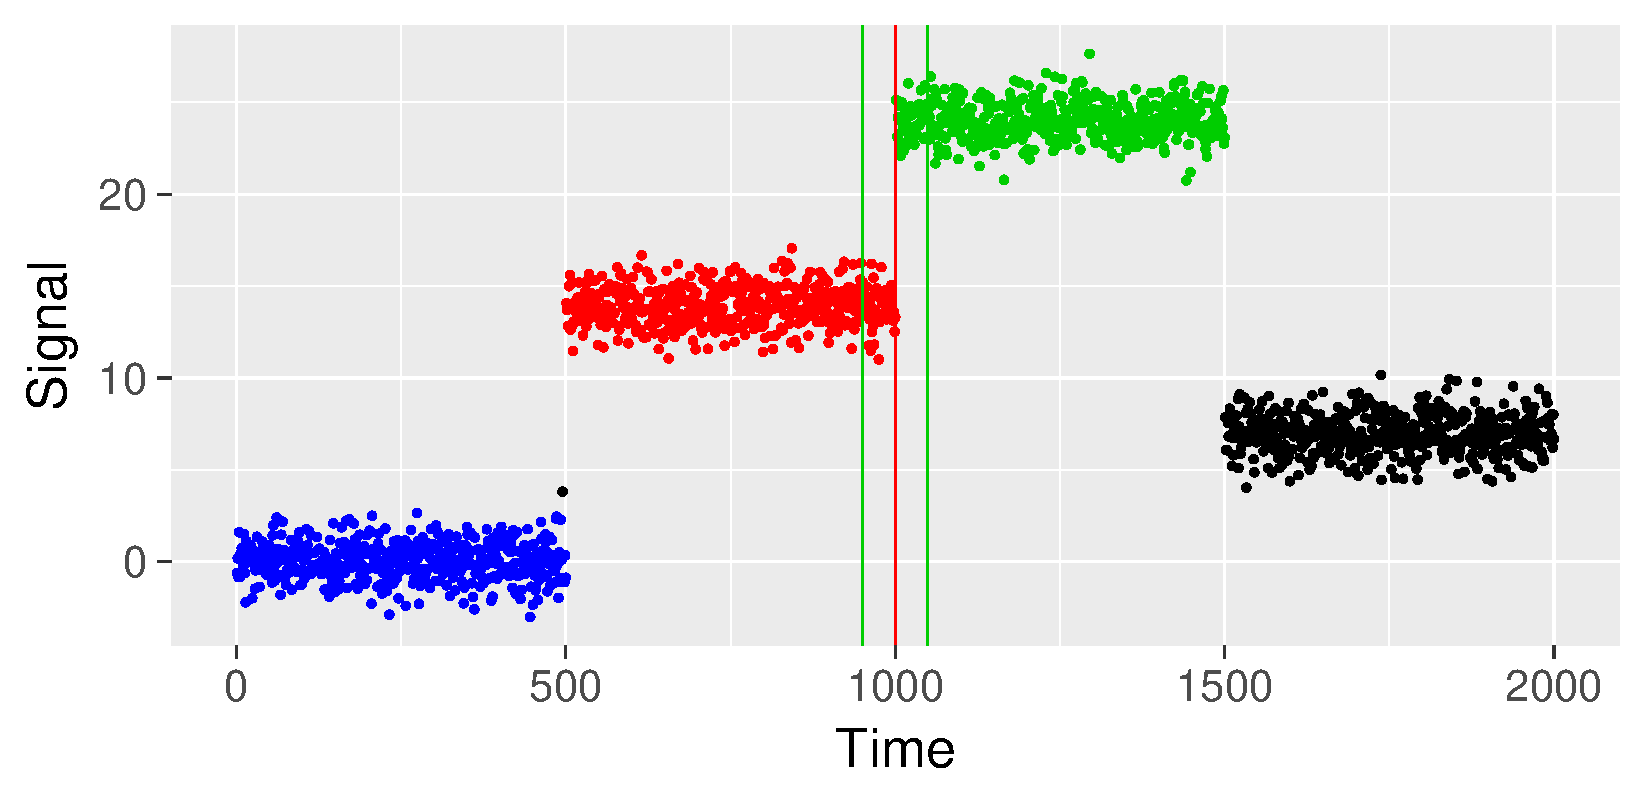
\includegraphics[width = \textwidth]{cim_7_new}
  \caption{$\tau = 1000 $, $\gamma = 50.$}
  \label{fig:cim_7}
  \end{subfigure}
  \caption{Example of searching for boundary locations on a simple change in mean example. The value of $\tau$ is given by the vertical red line, and the green lines show $\tau  - \gamma$ and $\tau + \gamma - 1$.}
  \label{fig:change_in_mean}
\end{figure}

In Figure \ref{fig:cim_6}, $\tau = 700$ and we can see that the 50 points before $\tau$ are assigned to the same cluster as the 50 points after $\tau$. This implies that $\tau$ is not a likely to be a boundary location. In Figure \ref{fig:cim_7}, $\tau = 1000$ and we can see that the 50 points before $\tau$ are mostly different in colour to the 50 points after $\tau$. This implies that $\tau$ is likely to be a good boundary location. In order to quantify this, we use a categorical similarity measure. To this end, we define the set $L$ to be the set of points to the left of $\tau$ given by $ L = \{x_{\tau - \gamma}, \ldots, x_{\tau -1}\}$. Similarly, we define the set $R$ to be the set of points to the right of $\tau$  given by $R = \{x_{\tau}, \ldots, x_{\tau + \gamma -1}\}$. In order to calculate how similar the cluster assignments of sets $L$ and $R$ are we calculate the following similarity metric. Let $n_{L,j}$ be the number of data points in set $L$ assigned to cluster $j$, where $j \in 1, \ldots, k$ and similarly for $n_{R,j}$. The categorical similarity metric is defined in equation \eqref{eq:sim_cont_tab}. This metric was inspired by the $\chi^2$ test statistic, although since the size of sets $L$ and $R$ are equal we can use a related, more intuitive comparison. 

\begin{equation}
  \label{eq:sim_cont_tab}
  \text{sim}(\tau, \gamma) = \frac{\sum_{j = 1}^{k} \min (n_{L,j}, n_{R,j})}{\gamma}.
\end{equation}
 
Note that this categorical similarity measure will be bound between $0$ and $1$, where 0 indicates perfect dissimilarity and 1 indicates that the distribution of the sets is identical.  We can think of this similarity measure as an indicator of how likely $\tau$ is to be a boundary location. If $\text{sim}(\tau, \gamma) = 0$ then $\tau$ is very likely to be a boundary location. We search over all values of $\tau \in \{\gamma+1 :  N-\gamma+1\}$ and define the set of boundary locations $B$ to be the values of $\tau$ which satisfy $\text{sim}(\tau, \gamma) = 0 $. The whole procedure for Stage 2 is summarised in Algorithm \ref{alg:boundary_locations}. 

\begin{algorithm}
\caption{Stage Two: Identifying Boundary Locations}  
\begin{algorithmic}[1]
\REQUIRE Data points =  $\boldsymbol{x_1} \ldots \boldsymbol{x_N}$, micro-cluster centres, number of macro-clusters $k$, search parameter $\gamma$.
\ENSURE A set of boundary locations $B$.
\STATE Set $B = \emptyset$. 
\STATE Apply k-means on the micro-cluster centres.
\STATE Assign each data point in  $\{\boldsymbol{x_1} \ldots \boldsymbol{x_N}\}$ to a k-means macro-cluster.
\FOR {$\tau \in \{\gamma+1 :  N-\gamma+1\}$}
\STATE Calculate $n_{L,j}$ and $n_{R,j}$ for all $j \in \{1, \ldots, k\}$. 
\STATE Calculate $\text{sim}(\tau, \gamma) = \frac{\sum_{j = 1}^{k} \min (n_{L,j}, n_{R,j})}{\gamma}$. 
  \IF{$\text{sim}(\tau, \gamma) = 0$}
   \STATE $B$ = $B \cup \tau$ .
  \ENDIF
\ENDFOR
\end{algorithmic}
\label{alg:boundary_locations}
\end{algorithm}

The number of boundary locations  identified  given by $|B|$  will depend on the choice of $k$ in the k-means clustering and the value of $\gamma$ selected. Generally, the smaller the value of $\gamma$, the more boundary locations will be identified. By searching over a range of values of $\gamma$ and $k$ this will give engineers a number of possible options of boundary locations for their consideration. The effect of these parameters on performance is explored in the next section. 

\newpage
\section{Results on DAS data}
\label{sec:das_analysis}

We now explore the use of CluStream with Algorithm \ref{alg:boundary_locations} to identify the location of corrupted data within acoustic sensing data. The data stream we consider consists of 10000 data points (one second of data) and ten different series relating to different depths within the oil well. In order to compare performance of our algorithm we compare against a ground truth. The ground truth is shown in Figure \ref{fig:ground_truth_das} and consists of six manually chosen boundary locations. 

\begin{figure}[H]
  \centering
  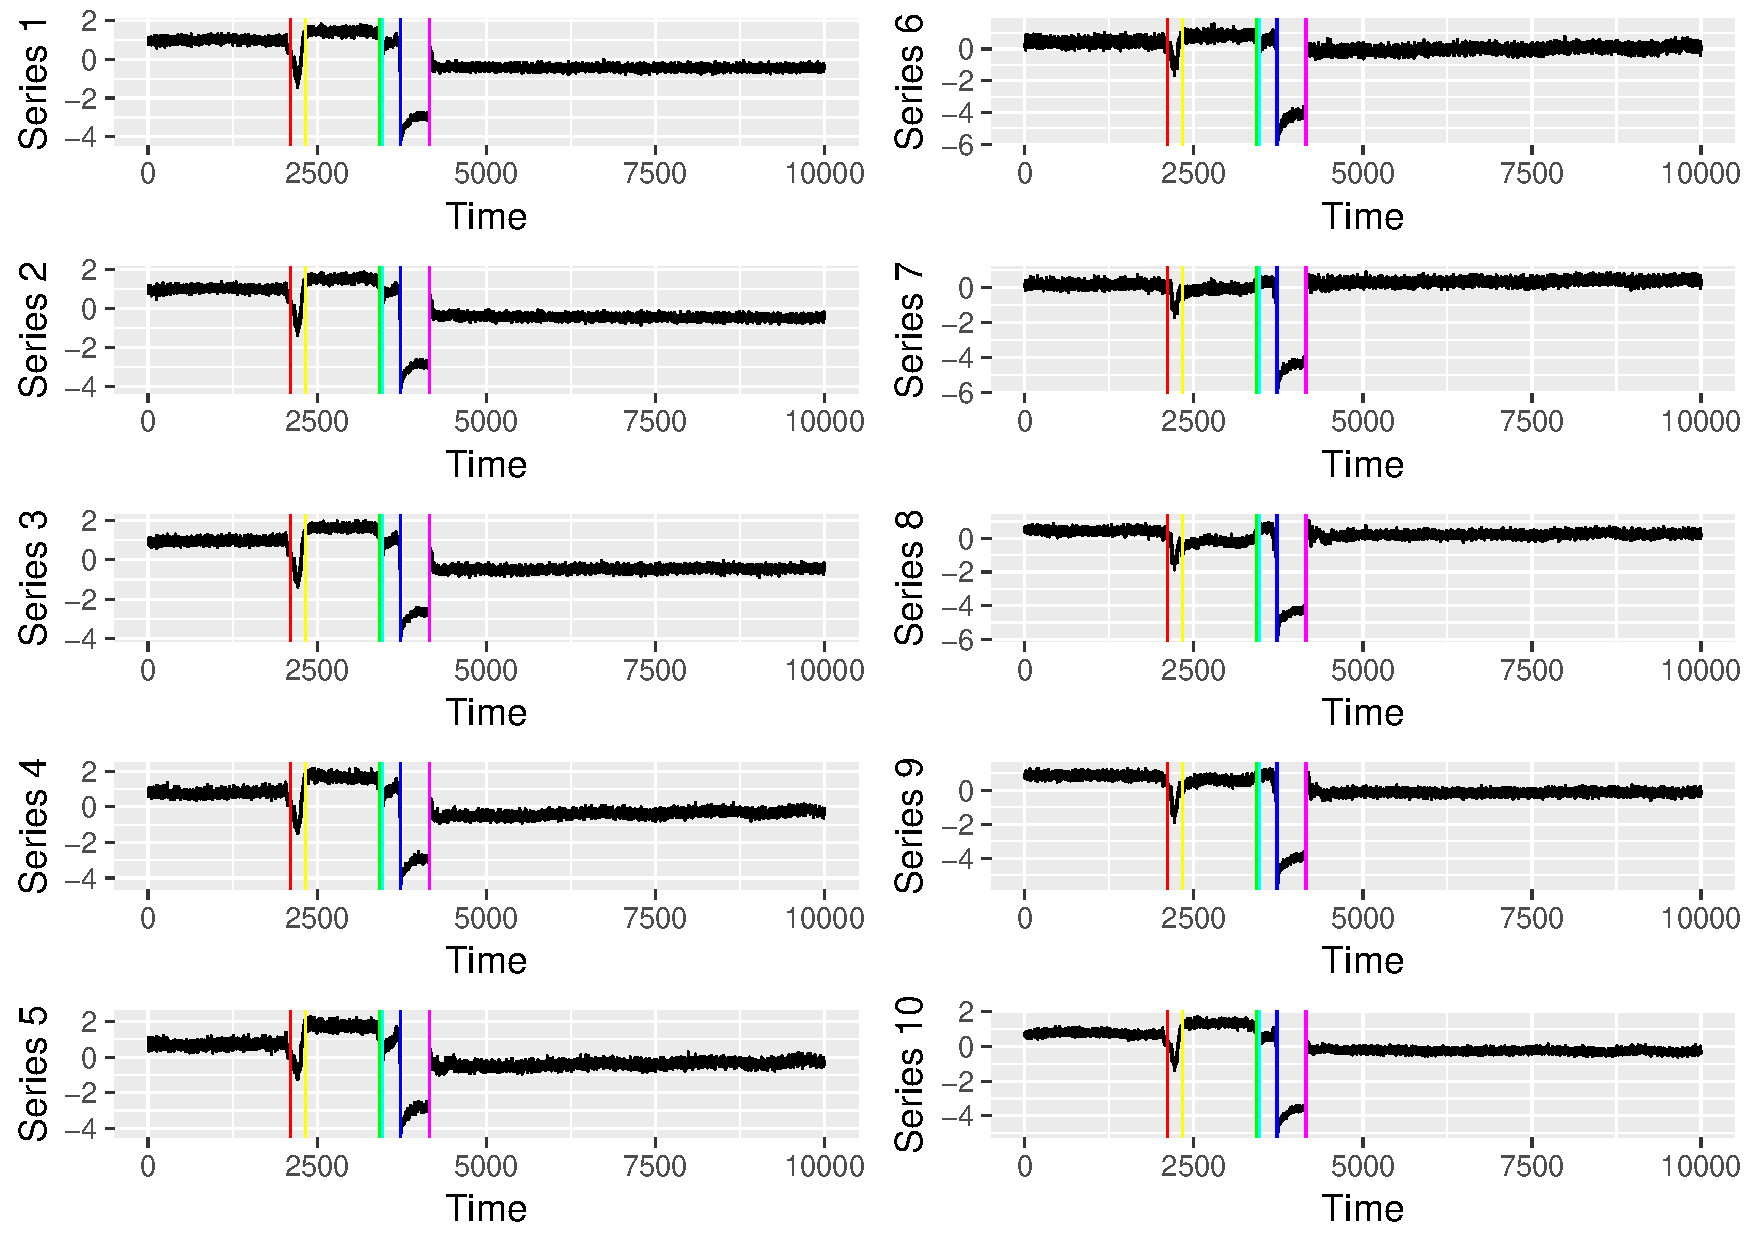
\includegraphics[width = 15cm]{ground_truth_new}
  \caption{Ground truth for the DAS data shown for all ten series. The six true boundary locations are shown with coloured vertical lines. }
  \label{fig:ground_truth_das}
\end{figure}

We compare the boundary locations found by Algorithm \ref{alg:boundary_locations} against the ground truth by using the V-measure. The V-measure \citep{Rosenberg2007} is a performance measure which rates the quality of a given segmentation compared to the ground truth segmentation. V-measure rates the segmentation by balancing both homogeneity and completeness.  A larger V-Measure value indicates higher accuracy, with a value of 1 indicating a perfect segmentation. For full details, see in Section \ref{sec:performance}.


CluStream was applied on the DAS data stream using 250 micro-clusters. At $t = 10000$ we applied Algorithm \ref{alg:boundary_locations} on the signal for a range of values of $k$ and $\gamma$ to identify boundary locations. Due to the randomness induced by the k-means step, the results for each experimental setting are averaged out over 10 runs. The variation between runs was minimal. The average V-measure for each setting is presented in Table \ref{tab:vmeasure_das}.

 \begin{table}[H]
 \centering
 \begin{tabular}{|l|llllllllll|}
 \hline
 \multicolumn{1}{|c|}{\multirow{2}{*}{$k$}} & \multicolumn{10}{c|}{$\gamma$} \\ \cline{2-11} 
 \multicolumn{1}{|c|}{} & 5 & 10 & 15 & 20 & 25 & 30 & 35 & 40 & 45 & 50 \\ \hline
 2 & \bftab 0.742 & \bftab 0.742  & \bftab 0.742 & \bftab 0.742 & \bftab 0.742 & \bftab 0.742 & \bftab 0.742 & \bftab 0.742 & \bftab 0.742 & \bftab 0.742 \\
 3 & \bftab 0.967 & 0.828 & 0.828 & 0.828 & 0.828 & 0.828 & 0.828 & 0.828 & 0.828 & 0.828 \\
 4 & \bftab 0.956 & 0.88 & 0.88 & 0.88 & 0.88 & 0.829 & 0.829 & 0.829 & 0.829 & 0.828 \\
 5 & 0.937 & 0.946 & \bftab 0.961 & \bftab 0.961 & \bftab 0.961 & 0.931 & 0.931 & 0.931 & 0.931 & 0.828 \\
 6 & 0.798 & 0.935 & \bftab 0.961 & \bftab 0.961 & \bftab 0.961 & 0.93 & 0.93 & 0.93 & 0.931 & 0.828 \\
 7 & 0.802 & 0.935 & 0.952 & 0.952 & \bftab 0.961 & 0.942 & 0.942 & 0.93 & 0.93 & 0.868 \\
 8 & 0.805 & 0.936 & 0.944 & 0.944 & \bftab 0.961 & 0.955 & 0.955 & 0.93 & 0.93 & 0.93 \\ \hline
 \end{tabular}
 \caption{V-measure results on the DAS data for a range of $k$ and $\gamma$. The best performance for each value of $k$ is highlighted in bold.}
 \label{tab:vmeasure_das}
 \end{table}

\newpage
The best performance in terms of V-measure is given by $k = 3$, $\gamma = 5$ however, good performance is found across the settings. The choice of $\gamma$ had no effect for the experiments where $k=2$. Generally as $k$ increases, the ideal choice of $\gamma$ for that value of $k$  also increases. This makes sense as when $k$ increases, $\text{sim}(\tau,\gamma)$ is more likely to take values of 0, resulting in more boundary locations being identified. By choosing a larger $\gamma$ for larger values of $k$, this prevents the number of boundary locations chosen by the algorithm from growing too large. The average number of boundary location identified by the algorithm under the different scenarios is given in Table \ref{tab:numLoc_das}.

\begin{table}[H]
\centering
\begin{tabular}{|l|llllllllll|}
\hline
 \multicolumn{1}{|c|}{\multirow{2}{*}{$k$}} & \multicolumn{10}{c|}{$\gamma$} \\ \cline{2-11} 
\multicolumn{1}{|c|}{} & 5 & 10 & 15 & 20 & 25 & 30 & 35 & 40 & 45 & 50 \\ \hline
2 &\bftab 2    & \bftab 2    &\bftab 2   &\bftab 2   &\bftab  2   &\bftab 2   & \bftab 2   &\bftab  2   &\bftab 2   & \bftab2   \\
3 & \bftab 6    & 3    & 3   & 3   & 3   & 3   & 3   & 3   & 3   & 3   \\
4 & \bftab 8    & 5    & 5   & 5   & 5   & 4   & 4   & 4   & 4   & 3   \\
5 & 11   & 8    & \bftab 7   & \bftab 7   & \bftab 7   & 6   & 6   & 6   & 6   & 5   \\
6 & 19   & 11   &\bftab  9   & \bftab 8   &\bftab  8   & 7   & 7   & 7   & 6   & 5   \\
7 & 18.8 & 11.6 & 9.6 & 9   & \bftab 8.6 & 8   & 8   & 7.6 & 7   & 6.4 \\
8 & 18.4 & 11.6 & 9.6 & 9.4 & \bftab 8.6 & 8.4 & 8.4 & 7.6 & 7.4 & 7.4 \\ \hline
\end{tabular}
\caption{Average number of boundary locations identified on the DAS data for a range of $k$ and $\gamma$. The number of boundary locations corresponding to the best performing V-measure for each value of $k$ is highlighted in bold. The ground truth has $|B|=6$.}
\label{tab:numLoc_das}
\end{table}

\newpage
In Table \ref{tab:numLoc_das} we can see that the the number of boundary locations found does vary with $k$ and $\gamma$. However, the actual boundary locations identified are similar across the different parameter settings. In order to demonstrate this, Figure \ref{fig:best_k_gamma} plots the boundary locations identified using the most suitable value of $\gamma$ for each value of $k$. 

\begin{figure}[H]
  \centering
  \begin{subfigure}{0.45\textwidth}
    \centering
    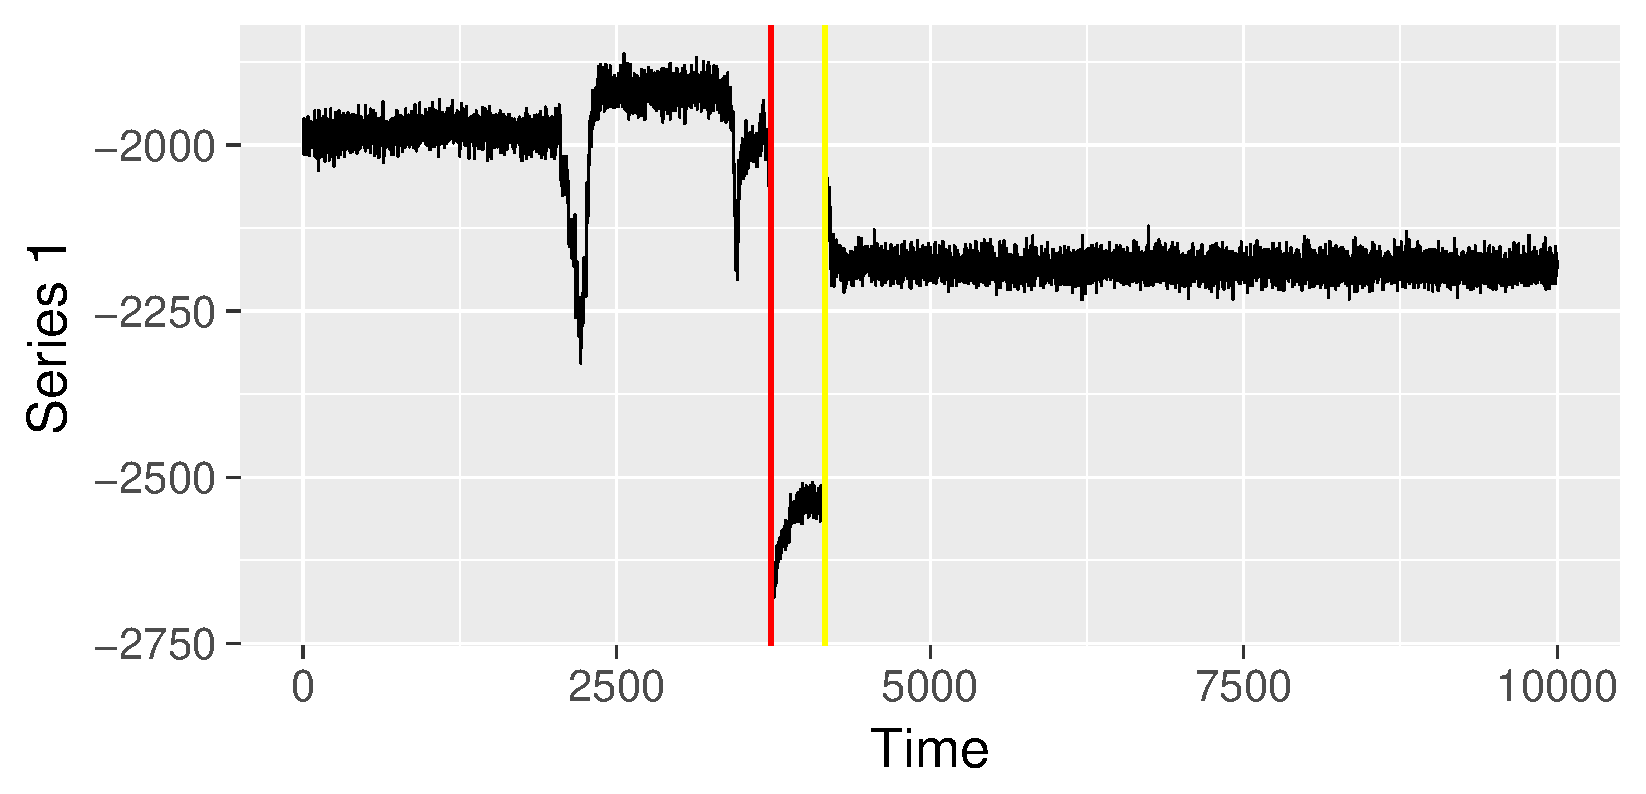
\includegraphics[width = \textwidth]{best/best_k_2_gamma_5_colour.pdf}
    \caption{$k = 2 $, $\gamma = 5$, $|B| = 2$.}
  \label{fig:best_2}
  \end{subfigure}
 \begin{subfigure}{0.45\textwidth}
    \centering
    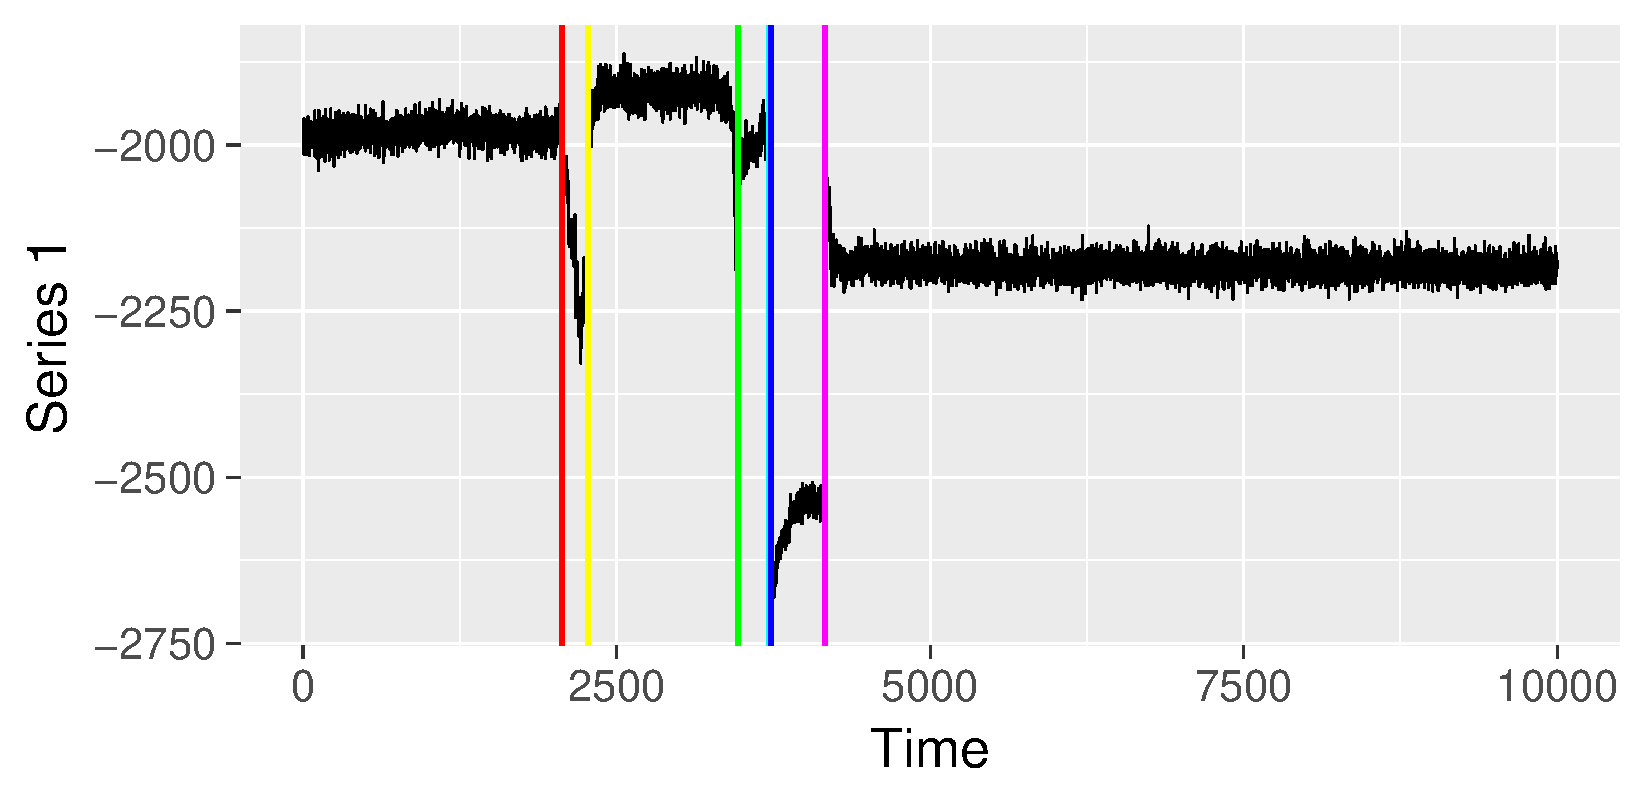
\includegraphics[width = \textwidth]{best/best_k_3_gamma_5_colour.pdf}
    \caption{$k = 3 $, $\gamma = 5$, $|B| = 6$.}
  \label{fig:best_3}
  \end{subfigure} \\

  \begin{subfigure}{0.45\textwidth}
    \centering
    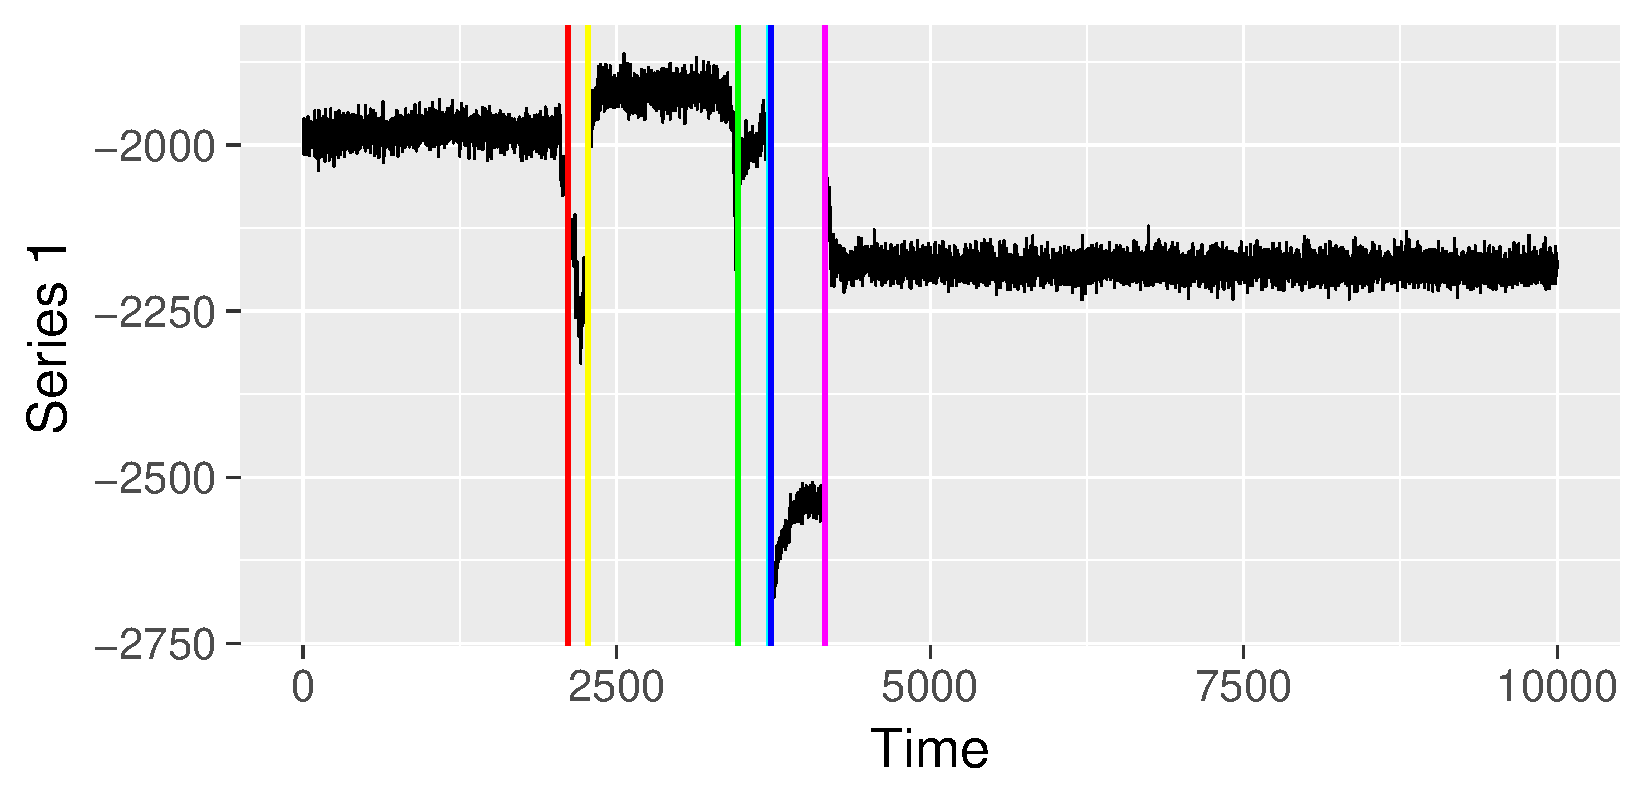
\includegraphics[width = \textwidth]{best/best_k_4_gamma_5_colour.pdf}
    \caption{$k = 4 $, $\gamma = 5$, $|B| = 8$.}
  \label{fig:best_4}
  \end{subfigure}
 \begin{subfigure}{0.45\textwidth}
    \centering
    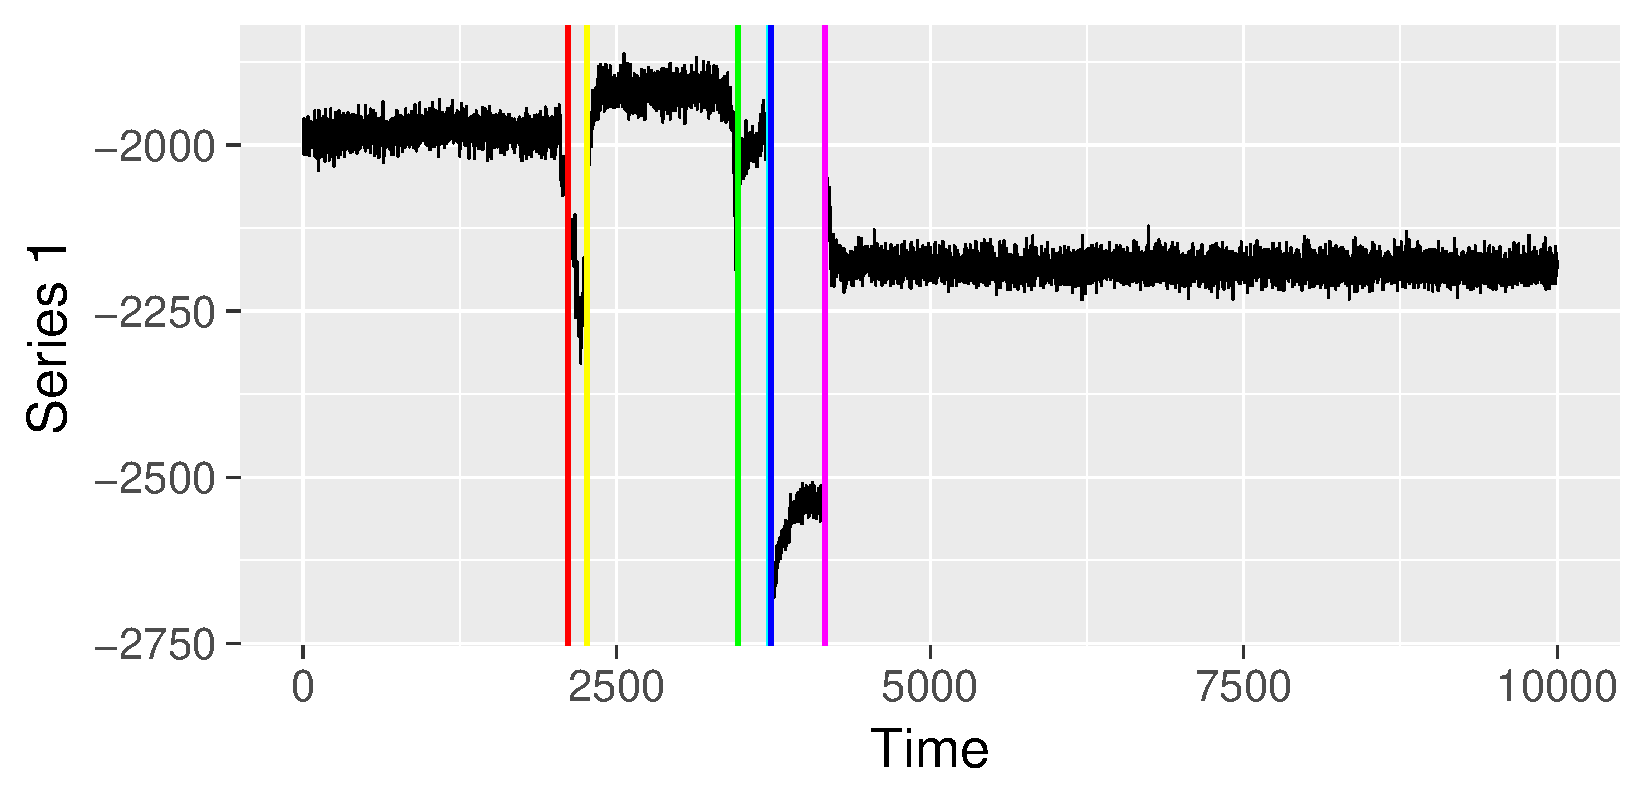
\includegraphics[width = \textwidth]{best/best_k_5_gamma_20_colour.pdf}
    \caption{$k = 5 $, $\gamma = 20$, $|B| = 7$.}
  \label{fig:best_5}
  \end{subfigure} \\

  \begin{subfigure}{0.45\textwidth}
    \centering
    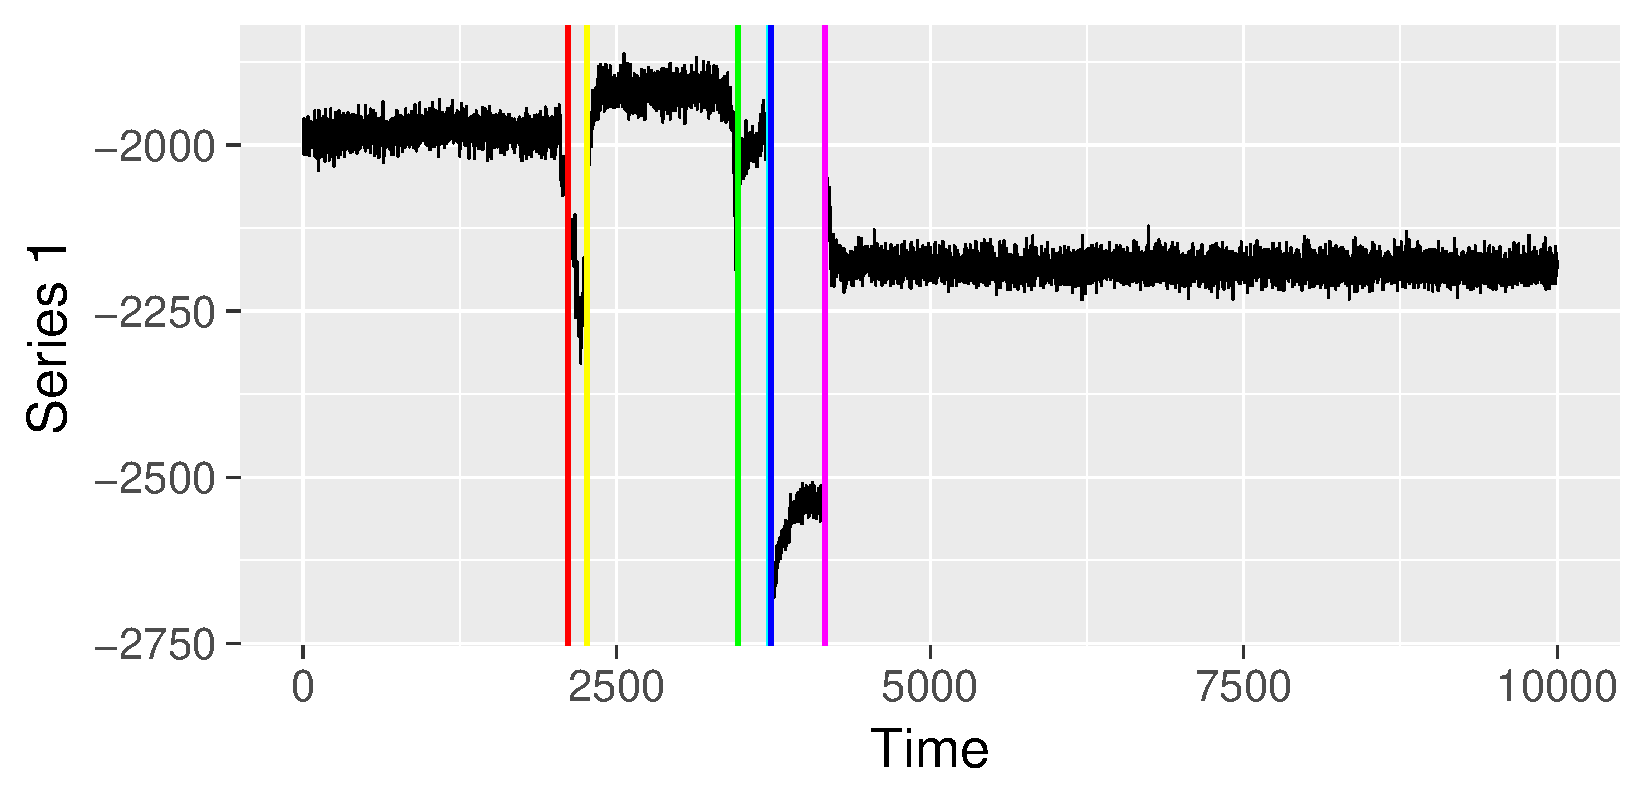
\includegraphics[width = \textwidth]{best/best_k_6_gamma_20_colour.pdf}
    \caption{$k = 6 $, $\gamma = 20$, $|B| = 8$.}
  \label{fig:best_6}
  \end{subfigure}
 \begin{subfigure}{0.45\textwidth}
    \centering
    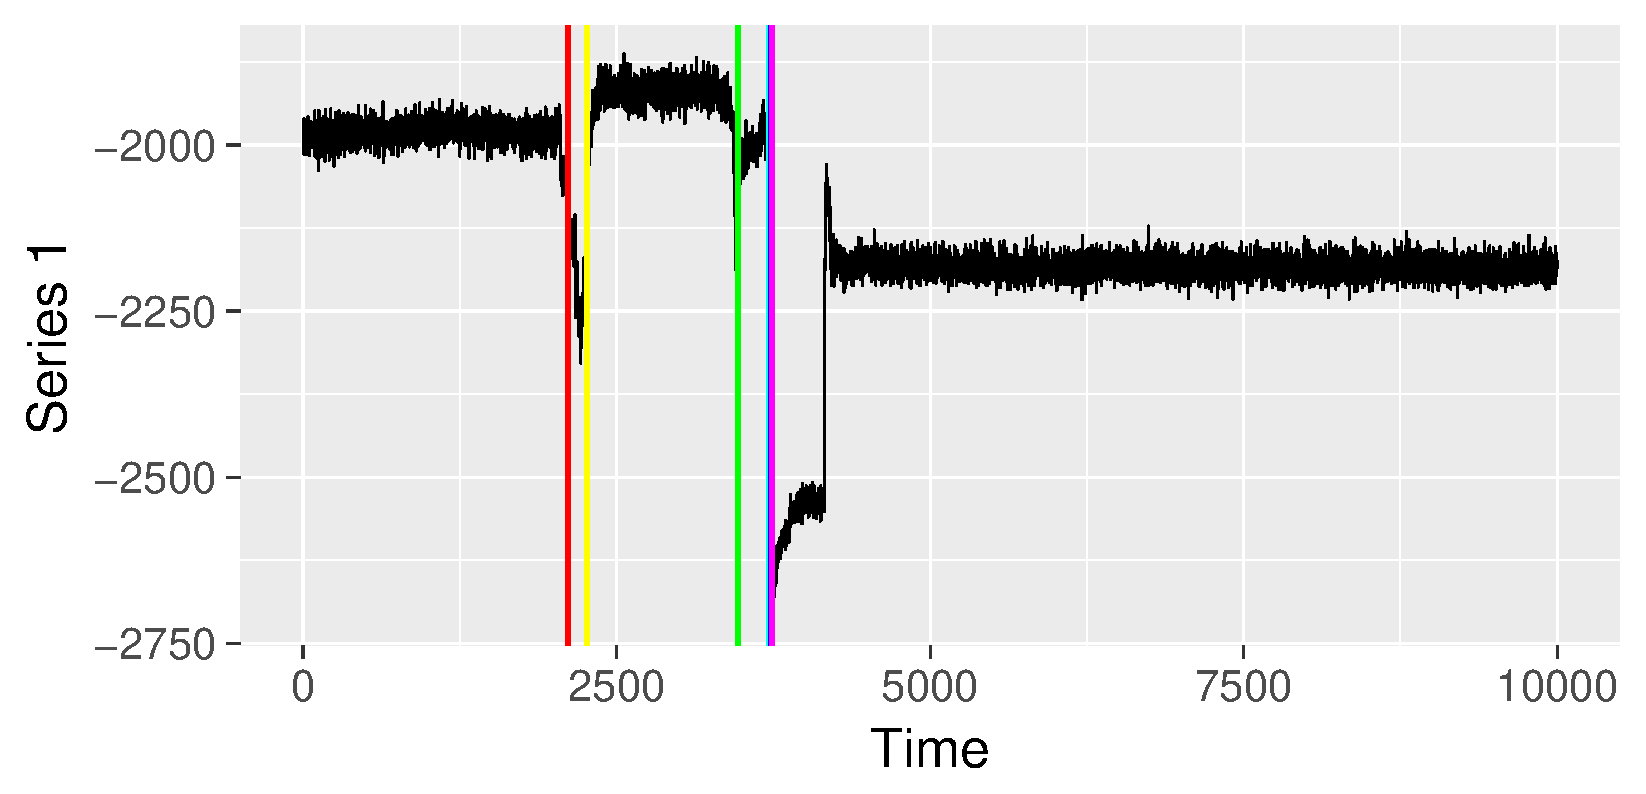
\includegraphics[width = \textwidth]{best/best_k_7_gamma_25_colour.pdf}
    \caption{$k = 7 $, $\gamma = 25$, $|B| = 9$.}
  \label{fig:best_7}
  \end{subfigure} \\

 \begin{subfigure}{0.45\textwidth}
    \centering
    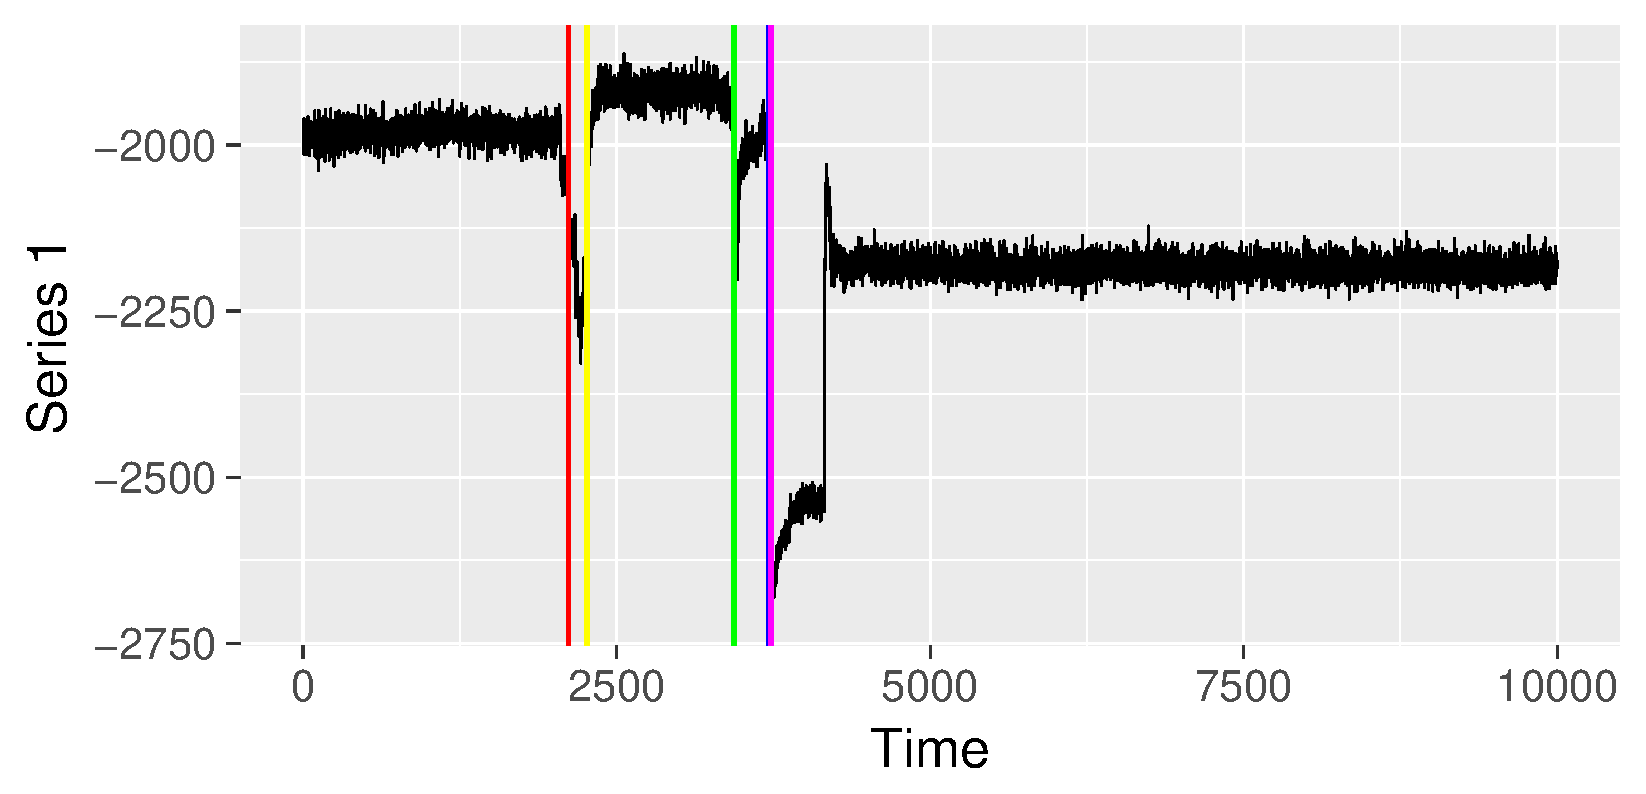
\includegraphics[width = \textwidth]{best/best_k_8_gamma_25_colour.pdf}
    \caption{$k = 8 $, $\gamma = 25$, $|B| = 9$.}
  \label{fig:best_8}
  \end{subfigure} \\
    \caption{Each plot shows the boundary locations (coloured lines) identified  under different parameter settings. We show one plot for each value of $k$, and use the most appropriate value of $\gamma$ in each setting. The number of boundary locations identified is given by $|B|$.}
  \label{fig:best_k_gamma}
\end{figure}

Only plots for Series 1 are shown in Figure \ref{fig:best_k_gamma} here but similar performance was observed across all ten series.  We can see that in Figure \ref{fig:best_2}, for $k=2$ only two boundary locations are found but these manage to pick out the most obvious data corruption. As $k$ increases, the number of boundary locations increases, but boundary locations only occur in places of change within the signal. For example, in Figure \ref{fig:best_8} we can see that $|B| = 9$ although we can only visibly see five red lines in the plot. This means that some of the boundary locations will be very close together, perhaps even neighbouring time points. 


\section{Conclusion}
\label{sec:das_conc}

In this chapter we have demonstrated that data summaries constructed by CluStream can help provide an alternative to changepoint detection methods for identifying corruption in digital acoustic sensing signals. The fact that CluStream can be run efficiently online means that it can cope well with the high frequency and high dimensionality data created by digital acoustic sensing. 

In order to frame the time-series as a clustering problem, we treated each time-series as a different data dimension. Interestingly the initial k-means clustering assignments look visually sensible in a temporal sense, despite no temporal information being given to the k-means algorithm.

We have developed an algorithm which uses a change in cluster assignments to identify boundary locations within the DAS signal. This algorithm was tested on the DAS data set for a range of values of $k$ and $\gamma$ and the results were found to be robust. As engineers are not clear exactly what defines a corrupted signal, offering a range of potential boundary locations by varying $\gamma$ and $k$ allows a set of solutions to be considered. 

When detecting boundary locations, we considered only the time points $\tau$ where $\text{sim}(\tau, \gamma)=0$. It would be possible to instead threshold $\text{sim}(\tau, \gamma)$  to increase the number of boundary locations identified by the algorithm. It would  also be possible to consider  $\text{sim}(\tau, \gamma)$ as a function of $\tau$ and treat identifying boundary locations as a local minima problem. However, we suspect that this would lead to many duplicate boundary locations being identified which would not be of use to the application. 
%The detection of changes in dependence structure is an important aspect of analysing many real-world time series, in particular acoustic sensing data.  estimating the number and locations of second-order changepoints.


 
%---------------- COMMENT FOR IMPORTING ----------------------
%\pagebreak											%Comment for importing
%\bibliographystyle{plainnat}		%Comment for importing
%\bibliography{References}				%Comment for importing
%\end{document}									%Comment for importing
%-------------------------------------------------------------



% Old boundary location notes
% When we wish to get the boundary locations the following steps are implemented.

% Use k-means as the macro-clustering step ($k$ is a user chosen parameter)
% This means applying k-means on the micro-cluster centers
% Assign all the data points in the series to a cluster, using the macro-clustering.
% List all of the cluster assignments temporally
% A boundary location is defined as anytime point where neighbouring points (in time) have different cluster assignments.  

%    A simple example is shown in Figure \ref{fig:change_in_mean}.

% \begin{figure}[H]
%   \centering
%   \begin{subfigure}{0.31\textwidth}
%     \centering
%     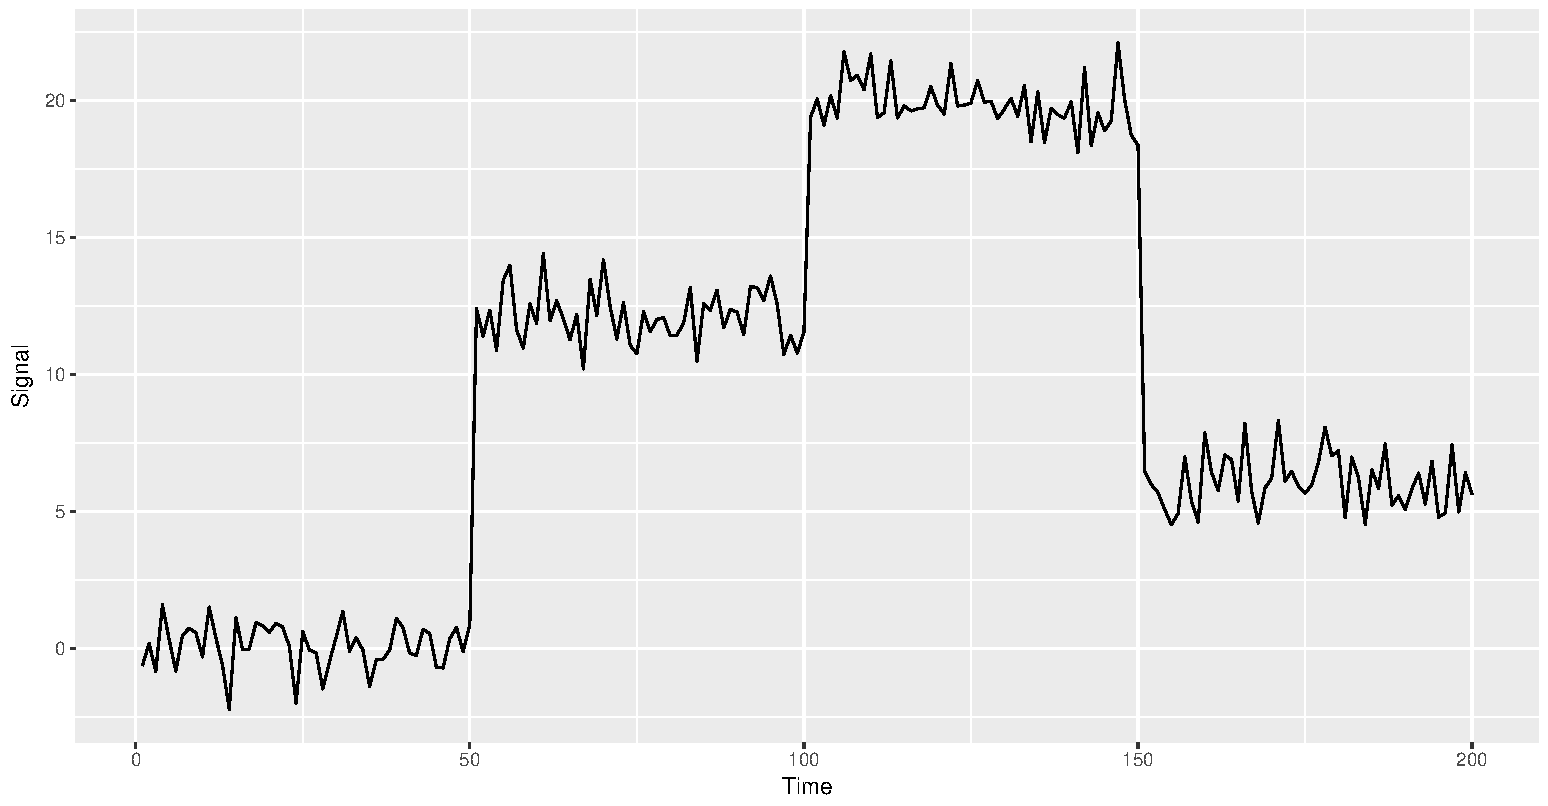
\includegraphics[width = \textwidth]{cim_1.pdf}
%     \caption{Original signal.}
%   \label{fig:cim_1}
%   \end{subfigure}
%   \begin{subfigure}{0.31\textwidth}
%     \centering
%     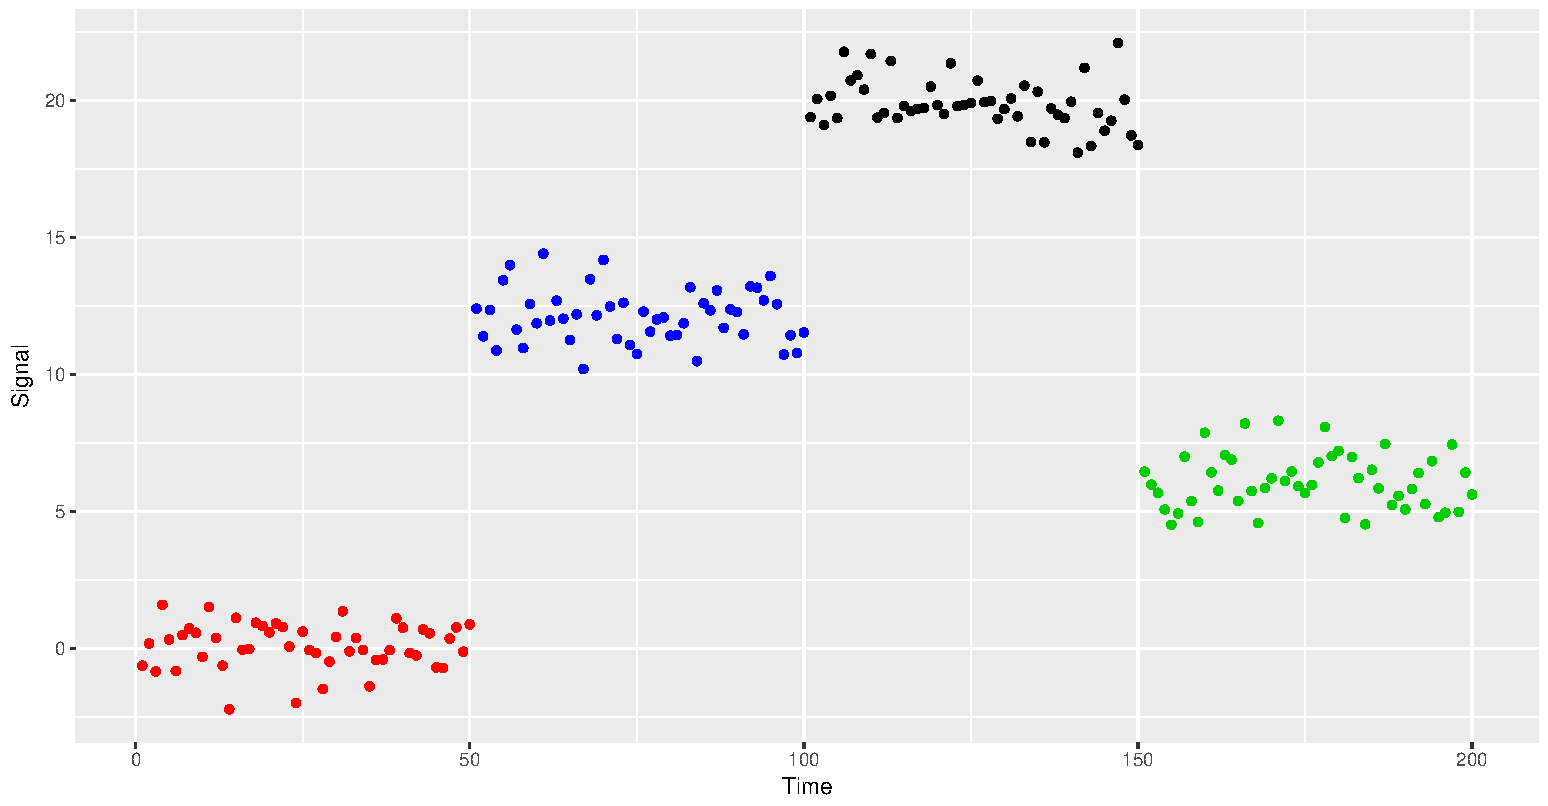
\includegraphics[width = \textwidth]{cim_2.pdf}
%   \caption{Clustering result.}
%   \label{fig:cim_2}
%   \end{subfigure}
%   \begin{subfigure}{0.31\textwidth}
%     \centering
%     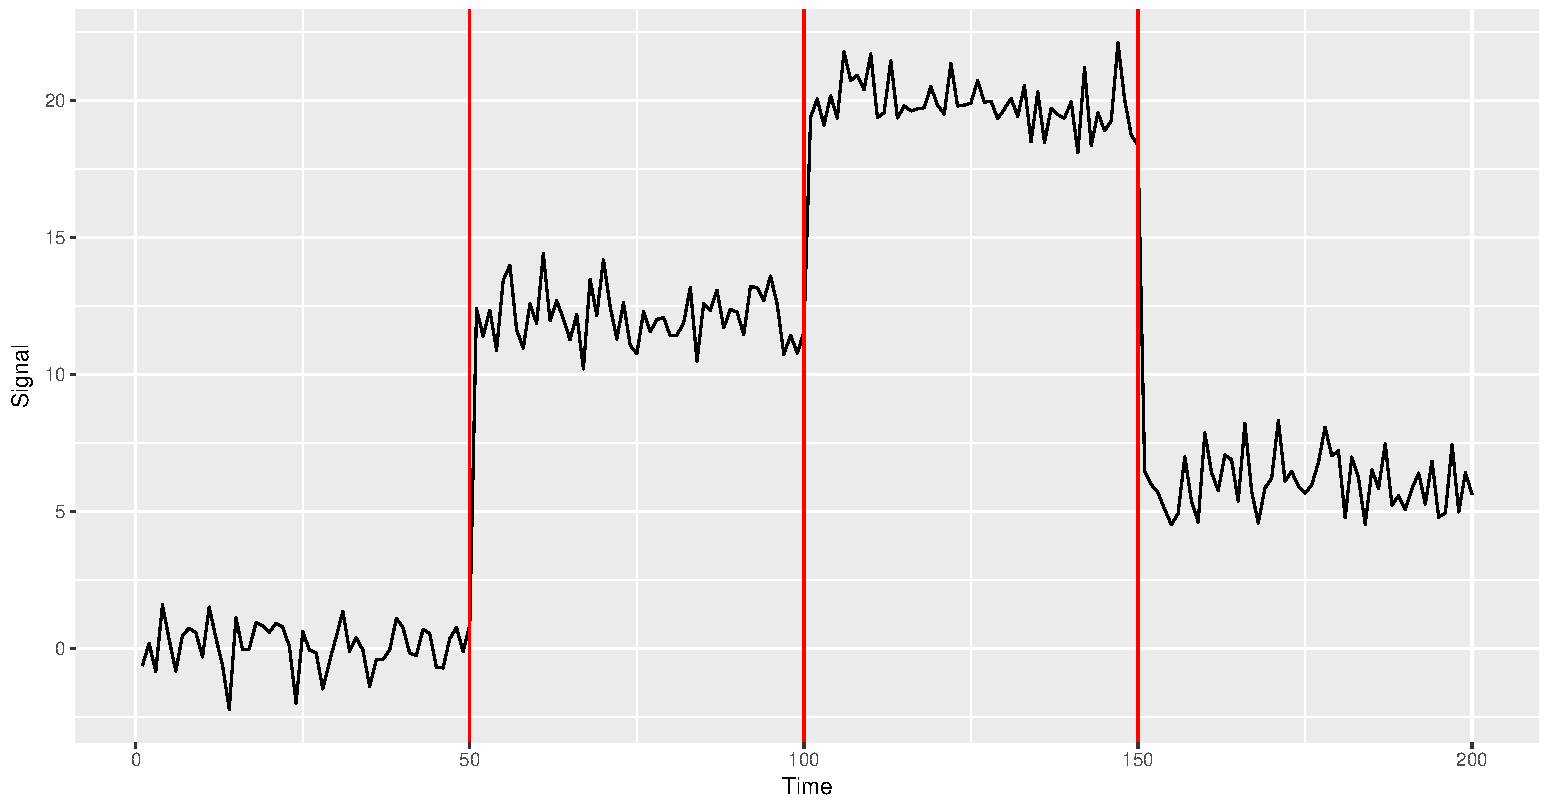
\includegraphics[width = \textwidth]{cim_3.pdf}
%   \caption{Estimated boundaries.}
%   \label{fig:cim_3}
%   \end{subfigure}
%   \caption{Example of segmentation generation on a simple change in mean example.}
%   \label{fig:change_in_mean}
% \end{figure}

% The estimated boundary locations given in Figure \ref{fig:cim_3} are drawn whenever the cluster label changes in time, correctly identifying the underlying change in structure in the signal.  

% By estimating the boundary locations in this way, we do not directly force there to be a particular number of boundary locations. The choice of $k$ in the k-means step will certainly influence the number of boundary locations identified, but this will not necessary be the same as the number of boundary locations identified.  To avoid an excessive number of boundary locations being identified, a post-processing step is implemented on the boundary locations. A boundary location is only identified if the new cluster assignment is observed for at least $\gamma$ time steps, where $\gamma$ is a user-chosen parameter. This will prevent boundary locations appearing when we observe an outlier rather than a true change in structure.  An example of this is shown in Figure \ref{fig:change_in_mean_post}. 

% The idea of a minimum run length is similar to the notion of having a minumum cluster size which is very common in clustering \citep{Everitt2001}. 

% \begin{figure}[H]
%   \centering
%   \begin{subfigure}{0.41\textwidth}
%     \centering
%     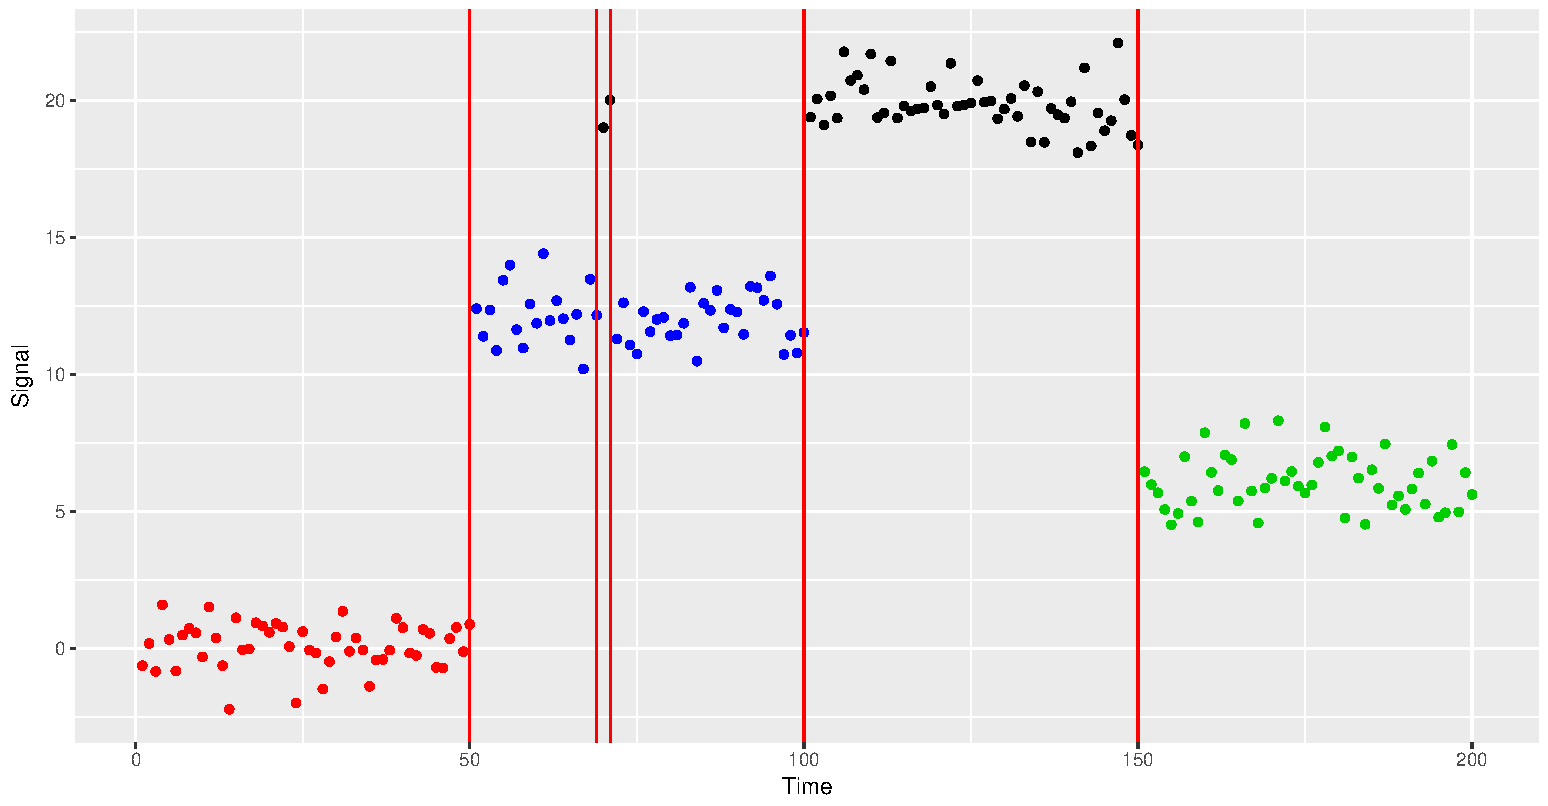
\includegraphics[width = \textwidth]{cim_4.pdf}
%     \caption{Without post-processing.}
%   \label{fig:cim_4}
%   \end{subfigure}
%   \begin{subfigure}{0.41\textwidth}
%     \centering
%     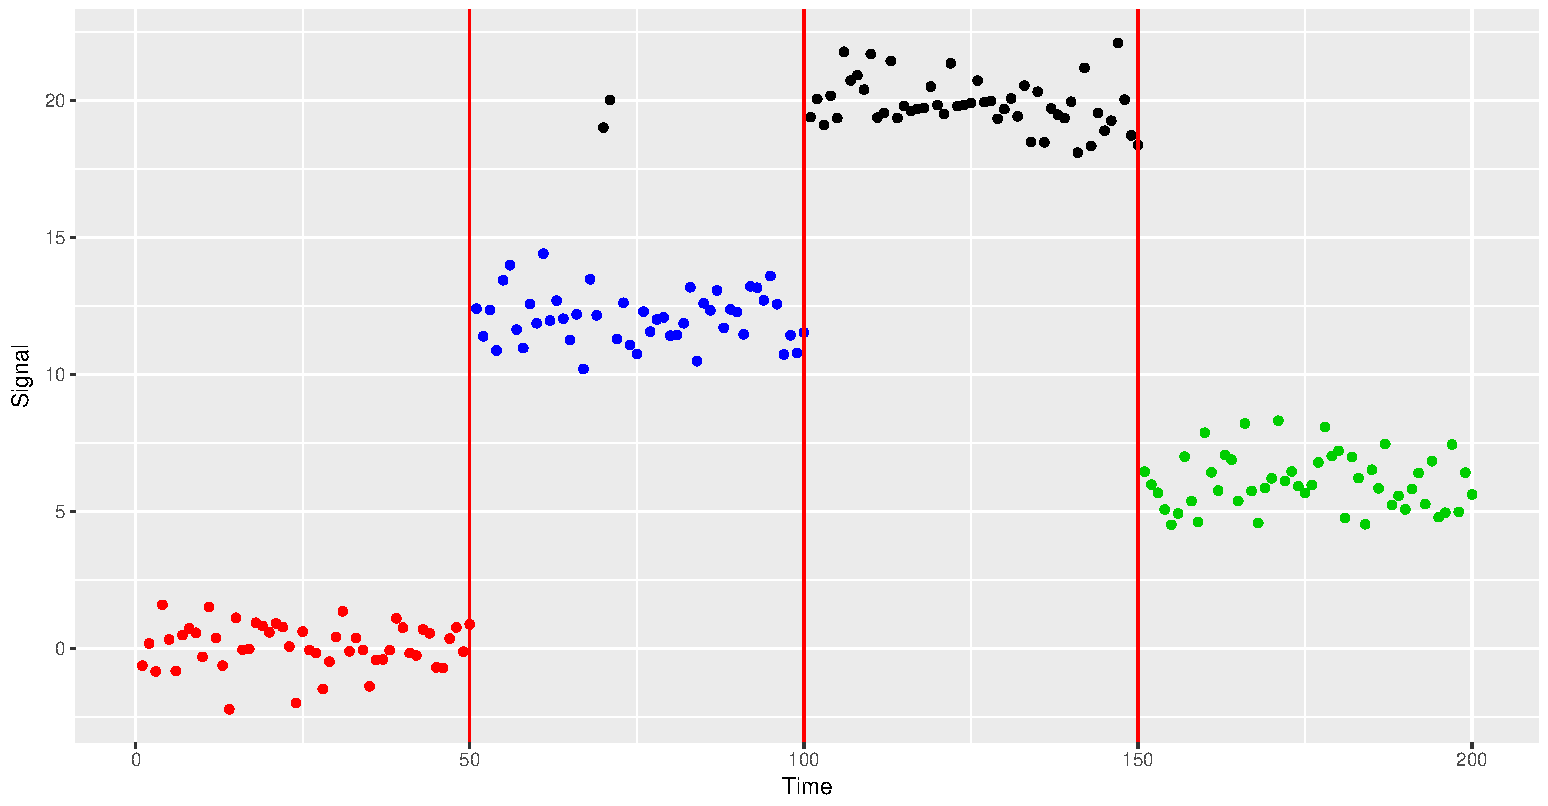
\includegraphics[width = \textwidth]{cim_5.pdf}
%   \caption{With post-processing.}
%   \label{fig:cim_5}
%   \end{subfigure}
%   \caption{Example of boundary location post-processing step.}
%   \label{fig:change_in_mean_post}
% \end{figure}

% The data in Figure \ref{fig:change_in_mean_post} is a similar data set to Figure \ref{fig:change_in_mean} but with 2 outliers occurring in the second segment. Without the boundary post-processing (Figure \ref{fig:cim_4}) boundary locations are estimated around the outliers.  With the boundary post-processing (Figure \ref{fig:cim_5}) only boundary locations which actually relate to a true change in underlying structure remain. 



%%%%%%%%%% OLD RESULTS


% \begin{figure}[H]
%   \centering
%   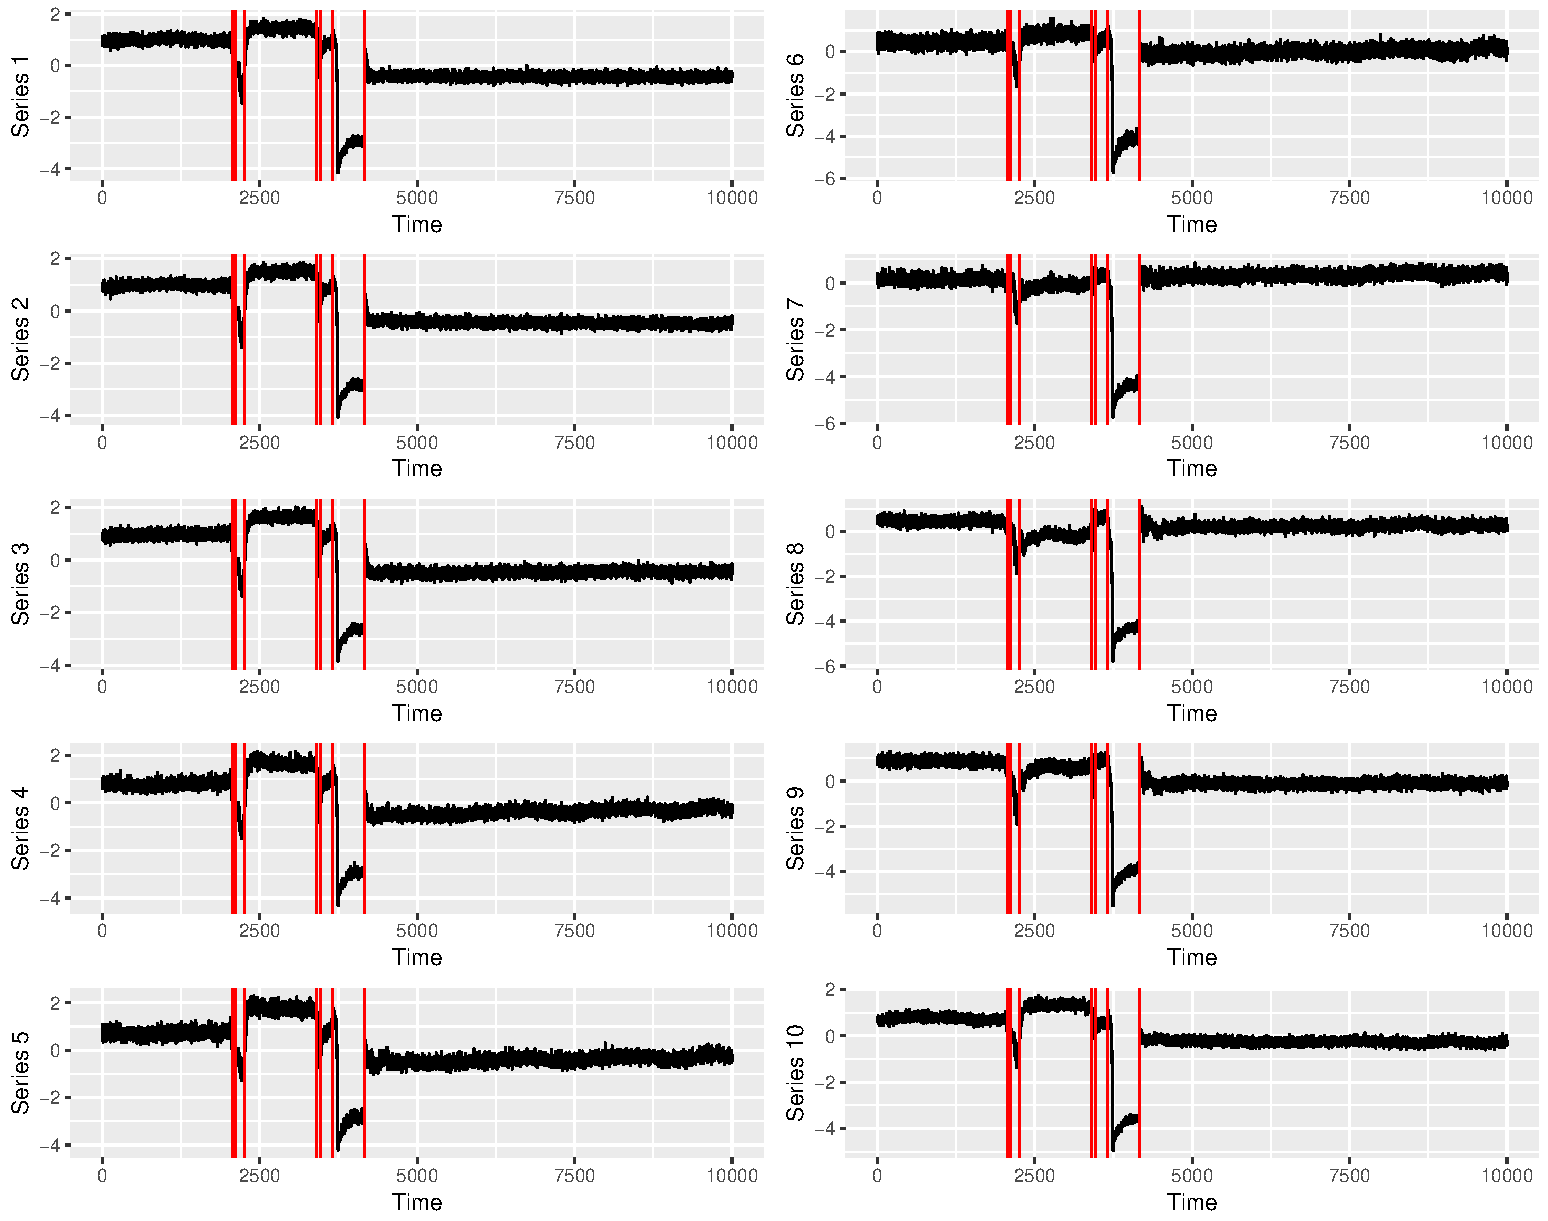
\includegraphics[width = 12cm]{10_channels/10_channels_end.pdf}
%   \caption{Segmentation using CluStream, red lines represent estimated boundary locations.}
%   \label{fig:das_clustream_segmented}
% \end{figure}

% Visual inspection of the results shows that CluStream provides a sensible segmentation of the data across all 10 series. Due to the nature of CluStream, the location of these boundaries are updated online. Figure \ref{fig:online_das_updates} demonstrates how the location of the boundaries is updated as the data stream progresses. 

% \begin{figure}[H]
%   \centering
%   \begin{subfigure}{0.31\textwidth}
%     \centering
%     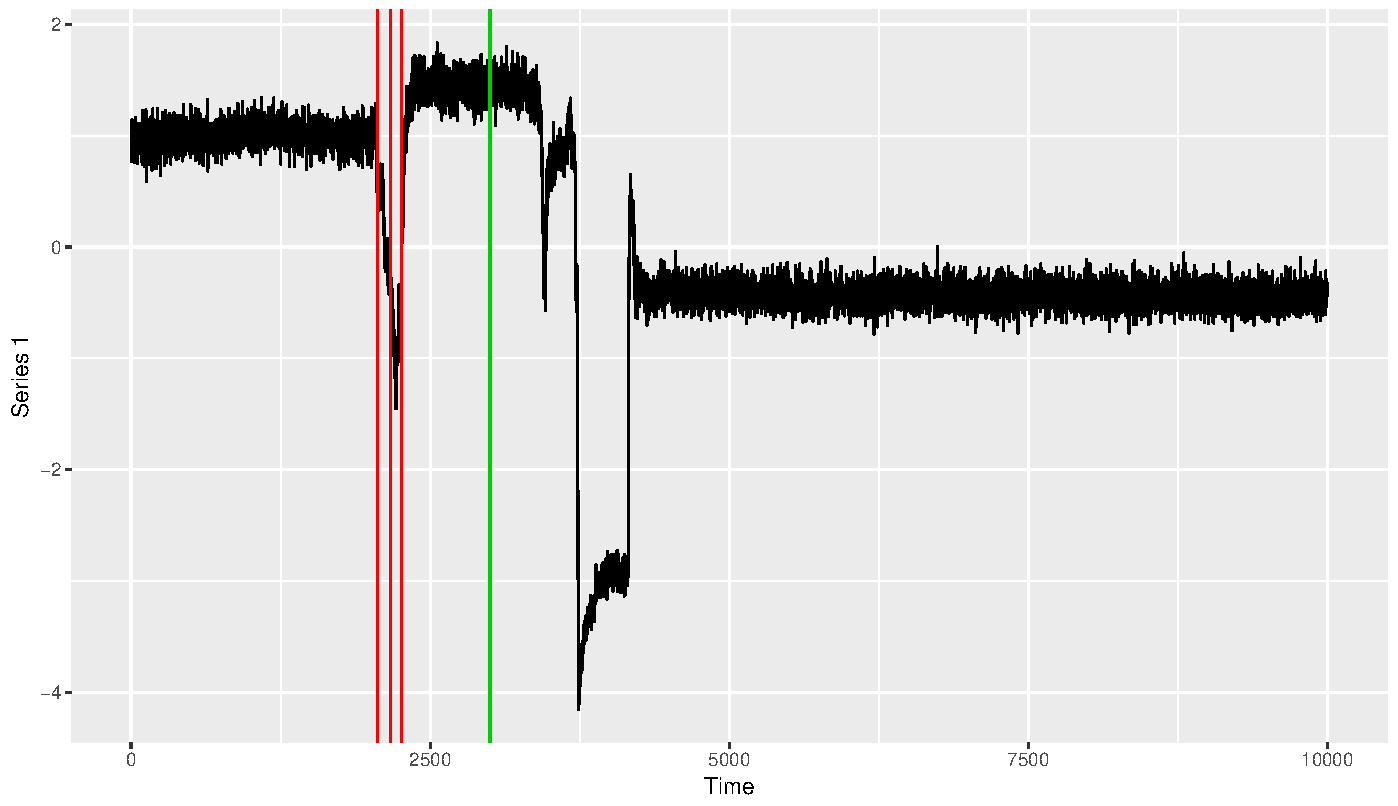
\includegraphics[width = \textwidth]{10_channels/10channels_time_3.pdf}
%     \caption{t = 3000}
%   \label{fig:das_4_3000}
%   \end{subfigure}
%   \begin{subfigure}{0.31\textwidth}
%     \centering
%     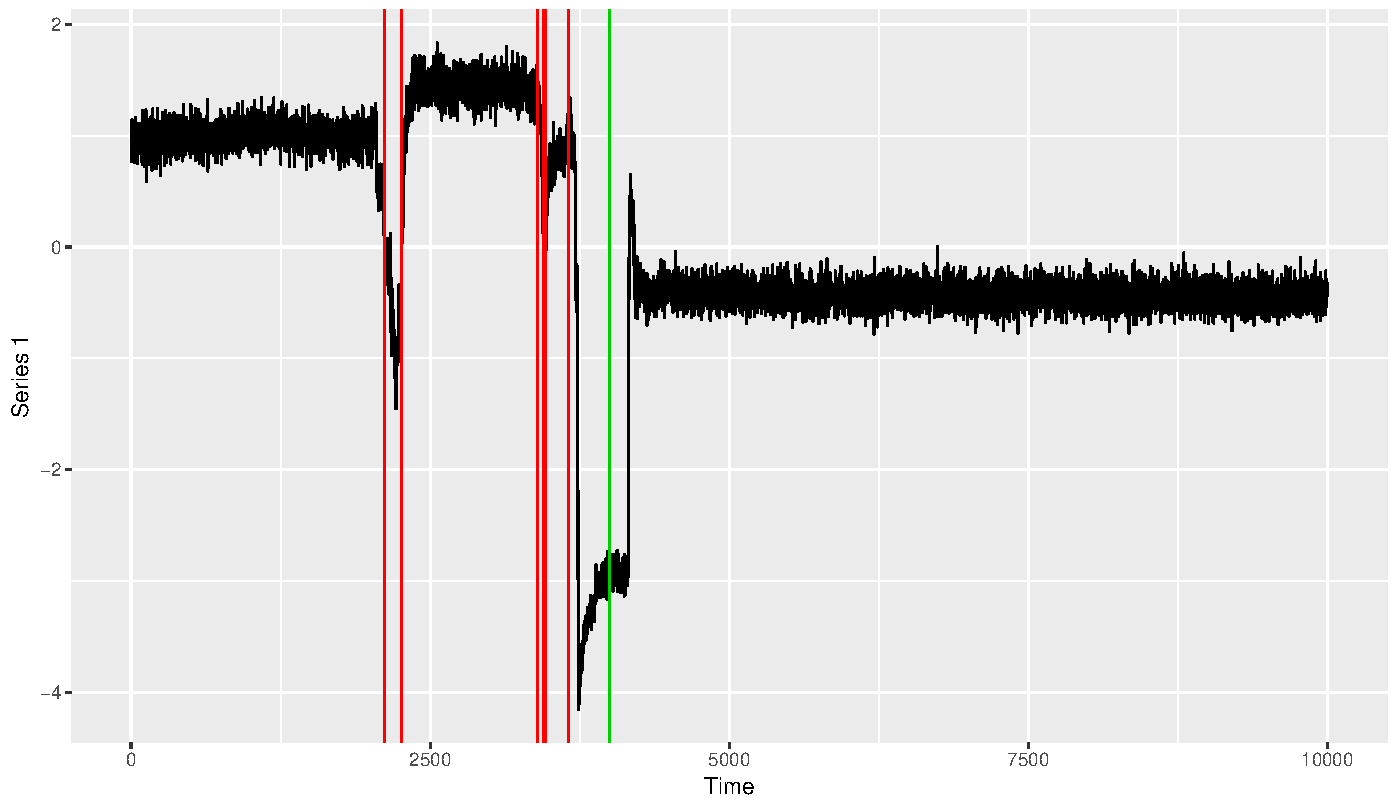
\includegraphics[width = \textwidth]{10_channels/10channels_time_4.pdf}
%   \caption{t = 4000}
%   \label{fig:das_t_4000}
%   \end{subfigure}
%   \begin{subfigure}{0.31\textwidth}
%     \centering
%     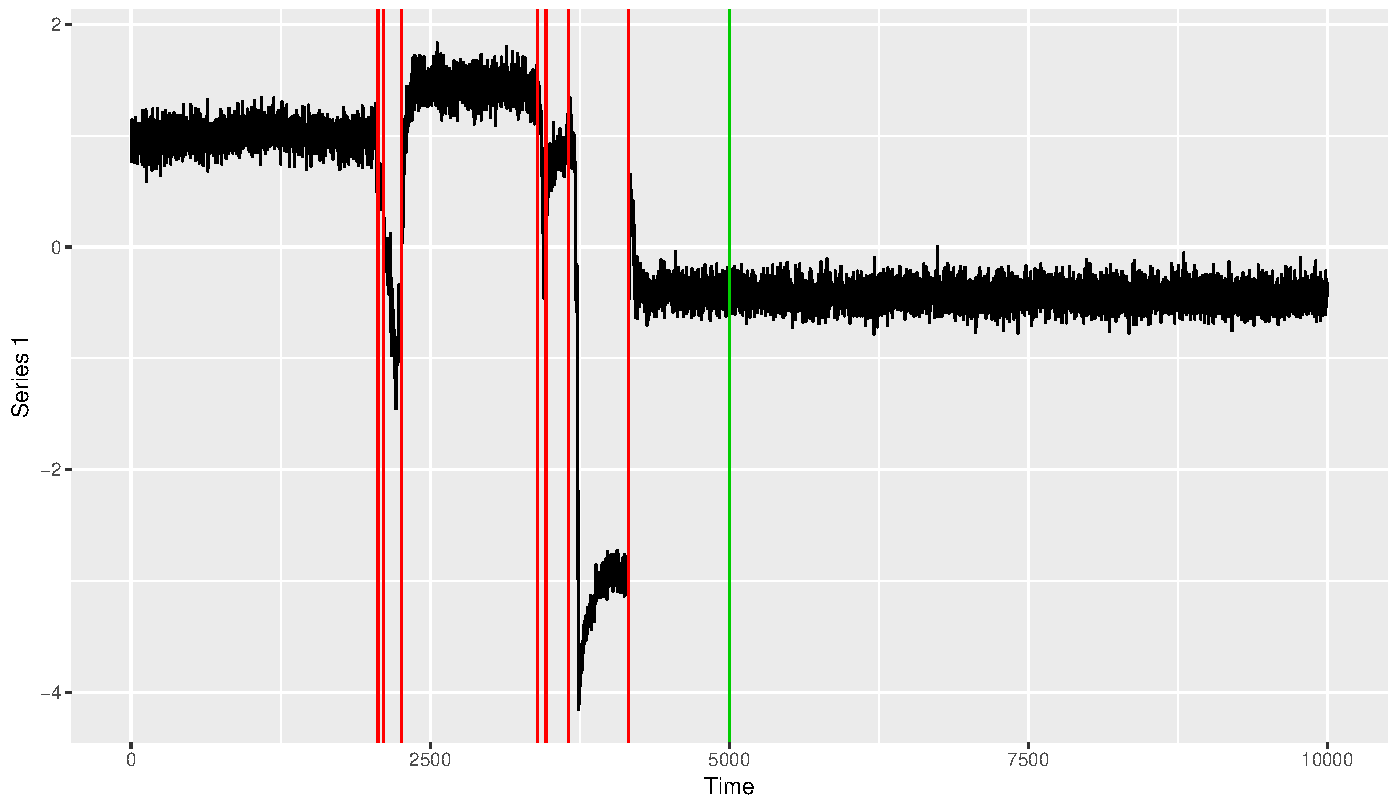
\includegraphics[width = \textwidth]{10_channels/10channels_time_5.pdf}
%   \caption{t = 5000}
%   \label{fig:das_t_5000}
%   \end{subfigure}
%   \caption{Updating the segmentation online.}
%   \label{fig:online_das_updates}
% \end{figure}

% In the plots, the estimated boundaries are given in red lines and the green line indicates how much of the signal has been observed so far. Only one of the ten series is shown for clarity. We can see that CluStream is quick to update the boundary locations estimates. This can be seen in Figure \ref{fig:das_t_4000}, where the change generated by the drop in the signal is identified after only a few hundred observations.

